% =============================================================================
% methods.tex  -  Methods of the Aim 4 parent marrow model (v1.3)
% Tables and numbers come from Code/config.R via make_tables.R:
%   Rscript Methods/make_tables.R && latexmk -pdf methods.tex   (in Methods/)
% =============================================================================
\documentclass[11pt]{article}
\usepackage[a4paper,margin=2.2cm]{geometry}
\usepackage[T1]{fontenc}
\usepackage{lmodern}
\usepackage{microtype}
\usepackage{amsmath,amssymb}
\usepackage{booktabs}
\usepackage{array}
\usepackage{xcolor}
\usepackage{tikz}
\usetikzlibrary{arrows.meta,positioning,calc}
\usepackage[font=small,labelfont=bf]{caption}
\usepackage[round,authoryear]{natbib}
\usepackage[hidelinks]{hyperref}
% generated by make_tables.R from Code/config.R - do not edit
\newcommand{\valThapCentre}{2.31}
\newcommand{\valThal}{1.05}
\newcommand{\valSrProg}{0.75}
\newcommand{\valKProg}{2}
\newcommand{\valEsr}{0.5}
\newcommand{\valEsrSd}{1}
\newcommand{\valStructSd}{0.5}
\newcommand{\valEtaCentre}{1}
\newcommand{\valEtaSd}{1.2}
\newcommand{\valAlcTarget}{0.042}
\newcommand{\valVOneNadir}{0.221}
\newcommand{\valRtol}{10^{-6}}
\newcommand{\valAtol}{10^{-9}}
\newcommand{\valHmax}{0.5}
\newcommand{\valDrvDt}{0.25}
\newcommand{\valDrvEnd}{130}
\newcommand{\valFerDecay}{0.07}
\newcommand{\valKernelH}{2}
\newcommand{\valTmin}{-31}
\newcommand{\valSetFrom}{-30}
\newcommand{\valSetTo}{-6}
\newcommand{\valWbcNoDiff}{0.5}
\newcommand{\valManualCells}{100}
\newcommand{\valGcsfDay}{14}
\newcommand{\valPltBelow}{30}
\newcommand{\valPltRise}{30}
\newcommand{\valHgbRise}{0.5}
\newcommand{\valPltDrop}{3}
\newcommand{\valObsMax}{120}
\newcommand{\valBrFrom}{2}
\newcommand{\valBrTo}{-7}
\newcommand{\valFerFrom}{-3}
\newcommand{\valFerTo}{35}
\newcommand{\valPhWin}{30}
\newcommand{\valNadFrom}{0}
\newcommand{\valNadTo}{14}
\newcommand{\valRec}{1.5}
\newcommand{\valDip}{1}
\newcommand{\valCensVal}{0.25}
\newcommand{\valPersFrom}{45}
\newcommand{\valPersTo}{75}
\newcommand{\valPersThr}{0.5}
\newcommand{\valItsMax}{12}
\newcommand{\valItsTol}{0.02}
\newcommand{\valStructEvery}{2}
\newcommand{\valOmegaNu}{4}
\newcommand{\valOmegaMax}{2.5}
\newcommand{\valMapMaxit}{150}
\newcommand{\valChains}{2}
\newcommand{\valIter}{1500}
\newcommand{\valBurn}{500}
\newcommand{\valThin}{2}
\newcommand{\valScale}{2.38}
\newcommand{\valAttrib}{400}
\newcommand{\valLandmarks}{0, 7, 10, 14, 21}
\newcommand{\valFDraws}{300}
\newcommand{\valFKernel}{200}
\newcommand{\valGcsfFold}{2.5}
\newcommand{\valTpoFold}{1.8}
\newcommand{\valNStates}{29}
\newcommand{\valNTrack}{19}
\newcommand{\valNPar}{66}
\newcommand{\valRVersion}{4.4.2}
\newcommand{\valVersion}{v1.3}
\newcommand{\valDEoptim}{2.2.8}
\newcommand{\valCarTzero}{0.001}
\newcommand{\valKag}{0.1}
\newcommand{\valKappa}{10.65}
\newcommand{\valKt}{0.2}
\newcommand{\valBetaA}{1}
\newcommand{\valKz}{0.5}
\newcommand{\valZfifty}{0.014}
\newcommand{\valThzs}{2.64}
\newcommand{\valEz}{0.5}
\newcommand{\valKg}{1}
\newcommand{\valGcsfRel}{2}
\newcommand{\valRhoCentre}{0.811}
\newcommand{\valRhoOmega}{0.5}
\newcommand{\valCartPeakDay}{8}
\newcommand{\valCartPeak}{0.05}
\newcommand{\valKernelA}{0.88}
\newcommand{\valKernelTp}{7.6}
\newcommand{\valCartPeakDayModel}{8}
\newcommand{\valCartPeakModel}{0.05}
\newcommand{\valZfiftyModel}{0.0141}
\newcommand{\valThzsModel}{2.63}
\newcommand{\valAucI}{12.3}
\newcommand{\valAucZ}{0.0939}
\newcommand{\valRouteLoss}{21.9}
\newcommand{\valThzsSd}{1}
\newcommand{\valEzSd}{1}
\newcommand{\valGcsfFoldLo}{1}
\newcommand{\valGcsfFoldHi}{10}
\newcommand{\valTauInit}{0.3}
\newcommand{\valTauMin}{0.02}
\newcommand{\valBoundSd}{4}
\newcommand{\valBoundMin}{1}
\newcommand{\valGcsfFrom}{15}
\newcommand{\valGcsfThr}{1}
\newcommand{\valGcsfDays}{5}
\newcommand{\valGcsfUntil}{100}
\newcommand{\valGcsfWin}{14}
\newcommand{\valGcsfPts}{10}
\newcommand{\valGcsfFlagged}{12}
\newcommand{\valGcsfNoWin}{2}
\newcommand{\valDeNp}{220}
\newcommand{\valDeF}{0.8}
\newcommand{\valDeCR}{0.9}
\newcommand{\valDeStrategy}{2}
\newcommand{\valDeChunk}{50}
\newcommand{\valDeWindow}{100}
\newcommand{\valDeTolBest}{10^{-6}}
\newcommand{\valDeTolSpread}{10^{-3}}
\newcommand{\valDeMaxGen}{20000}
\newcommand{\valDeStructNpMin}{60}
\newcommand{\valDeStructNpDim}{10}
\newcommand{\valDePolish}{500}
\newcommand{\valOutTolPar}{0.01}
\newcommand{\valOutTolObj}{10^{-4}}
\newcommand{\valOutNok}{2}
\newcommand{\valOutDamp}{0.5}
\newcommand{\valOutDampMin}{0.25}
\newcommand{\valOutMax}{120}
\newcommand{\valOutRelaxMin}{0.002}
\newcommand{\valOutRelaxAfter}{3}
\newcommand{\valOutRelaxGrow}{1.5}
\newcommand{\valOutLamMax}{10}
\newcommand{\valOutWindow}{10}
\newcommand{\valOutTolDrift}{0.02}
\newcommand{\valOutResetRise}{3}
\newcommand{\valOutMaxExtra}{0.5}
\newcommand{\valIsN}{2000}
\newcommand{\valIsNtwo}{4000}
\newcommand{\valIsDf}{4}
\newcommand{\valIsScale}{1.5}
\newcommand{\valIsEss}{30}
\newcommand{\valRhatTol}{1.05}
\newcommand{\valMcmcExtend}{1500}
\newcommand{\valMcmcMax}{9000}
\newcommand{\valEcores}{22}
\newcommand{\valMcores}{60}
\newcommand{\valRcohorts}{10}
\newcommand{\valRmodel}{MabC\_ddr}
\newcommand{\valRtruth}{$\theta_{zS}$ $\times2$, $e_Z$ $\times0.6$, $k_T$ $\times1.5$, $u_{\mathrm{R}}$ $\times0.7$, $\beta_A$ $\times0.7$, $e_{\mathrm{sr}}$ $\times0.8$}
\newcommand{\valWaveOne}{M0, Ma, Mb, Mab, Mabx, MF}


\newcommand{\dd}{\mathrm{d}}
\newcommand{\X}[1]{X_{\mathrm{#1}}}
\newcommand{\one}{\mathbb{1}}
\newcommand{\pos}[1]{\left(#1\right)_{+}}

\title{A lineage-resolved marrow model of blood count recovery after CAR T-cell therapy\\[4pt]
\large Model specification and statistical methods (Aim 4, model \valVersion)}
\author{Aim 4 working group, IMO Workshop 14}
\date{4 November 2026}

\begin{document}
\maketitle

\begin{abstract}
\noindent We describe a mechanistic model of haematopoiesis after lymphodepleting chemotherapy and CAR T-cell infusion. It is built to separate two axes of poor count recovery: \emph{who} (low marrow reserve versus a pre-existing haematopoietic clone) and \emph{when} (stem cell injury during bridging and lymphodepleting chemotherapy, ``a'', versus during the CAR T phase, ``b''). The haematopoietic hierarchy follows a stem cell (HSC) $\rightarrow$ multipotent progenitor (MPP) $\rightarrow$ common lymphoid / common myeloid progenitor (CLP / CMP) $\rightarrow$ granulocyte--monocyte / megakaryocyte--erythroid progenitor (GMP / MEP) tree with neutrophil, monocyte, megakaryocyte and lymphocyte outputs, and every self-renewing cell type carries its own self-renewal rate. In model version 1.3 the CAR T phase acts through two routes: the patient's measured ferritin course (marrow inflammation) and a mechanistic CAR T--target interaction, in which CAR T cells expand on CD19 antigen and generate a lagged signal that injures stem cells and suppresses MPP self-renewal; the CAR T cells add to the observed lymphocyte count. G-CSF is a model input, each patient's pre-treatment set points are individual parameters, and the population model is estimated by an iterative two-stage method in which every optimisation is a differential-evolution search with self-detected convergence. The model also tracks the mean time and the mean number of divisions since a cell entered the MPP compartment. This document gives every equation, the meaning of every term, all parameter values and their sources, the observation model, the estimation procedures, the pre-registered analysis plan and the verification of the implementation.
\end{abstract}

\tableofcontents
\clearpage

% -----------------------------------------------------------------------------
\section{Overview}

Time $t$ is in days relative to CAR T-cell infusion (day 0). Each patient is simulated from a pre-treatment steady state that starts at $t_0=\min(\valTmin,\ t_{\mathrm{aph}}+1,\ t_{\mathrm{first\,obs}}-1)$, where $t_{\mathrm{aph}}$ is the apheresis day. Every haematopoietic compartment is expressed relative to its own pre-treatment value, so all of them equal 1 at steady state; CAR T cells are counted in absolute units. The model has three layers (Figure~\ref{fig:tree}):
\begin{enumerate}
\item the \textbf{inputs}: the chemotherapy exposure $C(t)$ (``a''); the CAR T phase (``b''), which acts through the lagged ferritin-driven inflammation $I(t)$ and through the signal $Z(t)$ of a CAR T--target interaction module; and G-CSF, through its effect $E_G(t)$;
\item the \textbf{haematopoietic tree}: a two-clone HSC compartment, five self-renewing progenitor compartments (MPP, CMP, GMP, MEP, CLP), three maturation chains (neutrophil, monocyte, megakaryocyte) and a self-renewing lymphocyte pool;
\item the \textbf{blood}: absolute neutrophil, monocyte and lymphocyte counts (ANC, AMC, ALC) and platelets (PLT); the observed ALC is the sum of lymphocytes and CAR T cells.
\end{enumerate}
The parent model has \valNStates{} state variables (plus $2\times\valNTrack$ moment variables when ages and generations are tracked) and \valNPar{} parameters. The original Friberg myelosuppression model \citep{friberg2002} is implemented separately as the reference model MF (Section~\ref{sec:mf}).

\subsection{Changes from model v1.2}\label{sec:changes}
Model v1.2 and its pre-registered results are kept unchanged (frozen code, separate result folders). Version 1.3 changes the following:
\begin{enumerate}
\item \textbf{CAR T--target interaction} (Section~\ref{sec:cart}): CAR T cells $C_T$, CD19 antigen $A$ and a two-stage lagged interaction signal $Z$. $Z$ injures the HSC ($\theta_{zS}$, a second route of ``b'') and suppresses MPP self-renewal ($e_Z$). A new random effect, the expansion rate $\rho_T$, and ALC enters the likelihood as lymphocytes plus CAR T cells (v1.2: ALC not fitted).
\item \textbf{G-CSF as input} (Section~\ref{sec:gcsf}): the effect $E_G$ raises neutrophil chain entry and accelerates the release of mature neutrophils. Because only ``G-CSF needed after day 14'' is recorded, the dosing windows are imputed by a fixed rule. ANC values under G-CSF are ordinary observations (v1.2: upper bounds).
\item \textbf{Individual baselines} (Section~\ref{sec:baseline}): each lineage's set point is an individual parameter with a prior centred on the pre-treatment median; the rows that define the median enter only through this prior.
\item \textbf{Estimation} (Section~\ref{sec:its}): DE-ITS, an iterative two-stage method in which the individual and structural optimisations are differential-evolution searches inside a physiological search box, with self-detected convergence at every level (v1.2: BFGS and at most 12 iterations). The marginal likelihood for the BIC is computed by adaptive importance sampling (v1.2: Laplace).
\item \textbf{Model set}: route variants of the CAR T--target signal (HSC only, MPP only) and two waves of fits (Section~\ref{sec:nested}).
\item \textbf{Downstream analyses}: the landmark prediction keeps the population of the full-data fit (approximate, Section~\ref{sec:landmark}); the identifiability study K3 is replaced by a recovery test on synthetic cohorts (Section~\ref{sec:recovery}).
\end{enumerate}
Unchanged: the lineage tree and its self-renewal rates, the feedback structure, the ferritin route, the phenotype rule, the calibrations of $\theta_{aP}$, $\theta_{aL}$ and the progenitor self-renewal rate, and the numerical settings (driver grid \valDrvDt~d, maximal step \valHmax~d).

\begin{figure}[!htbp]
\centering
\resizebox{\textwidth}{!}{%
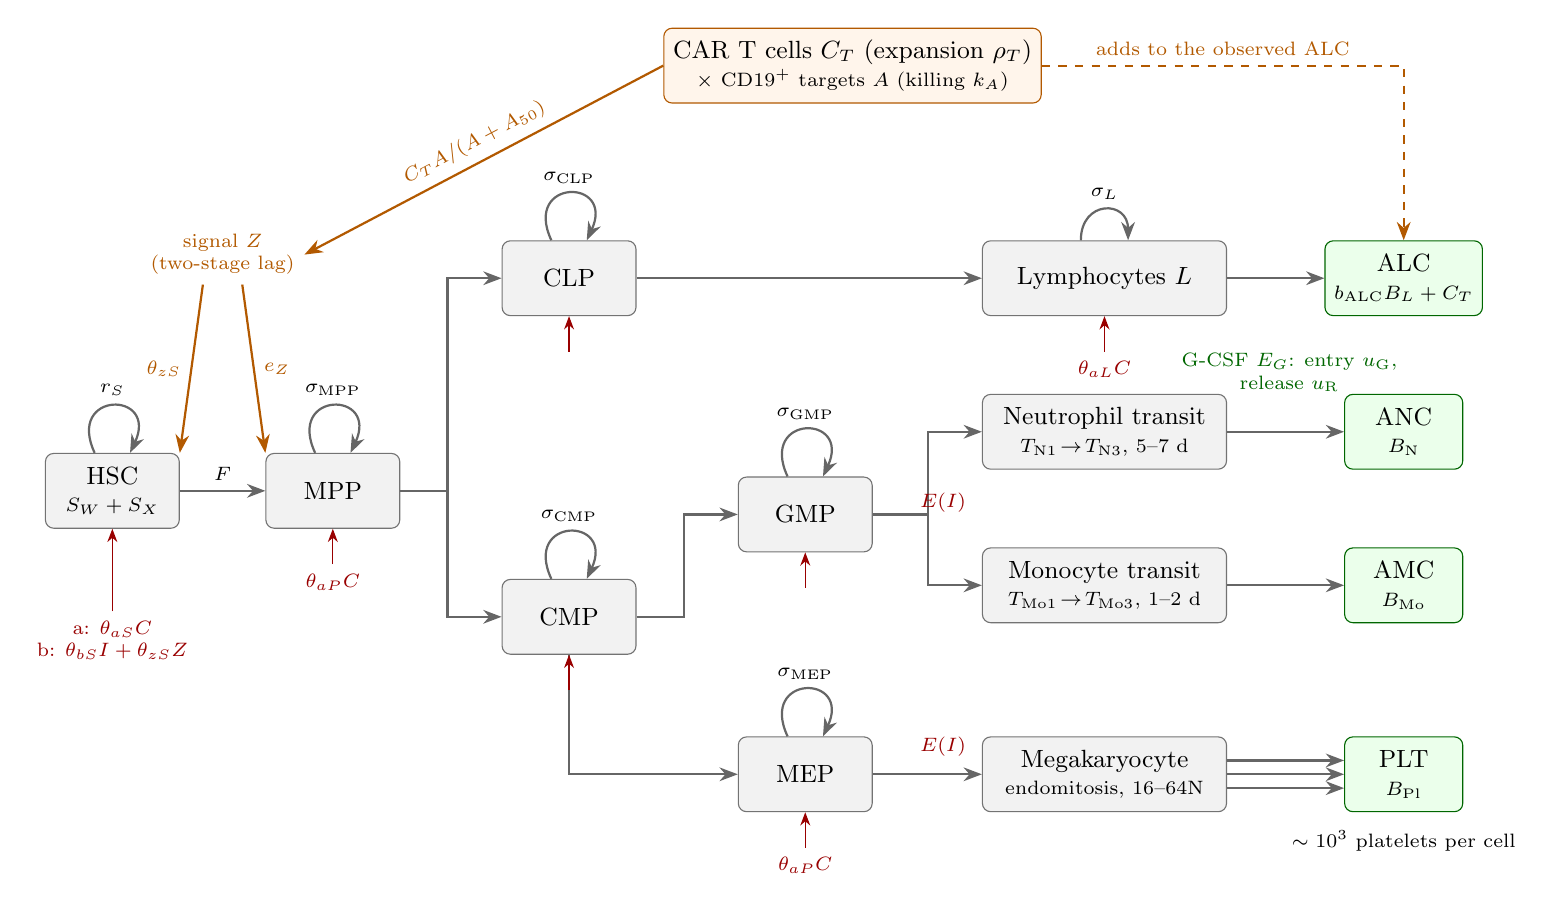
\begin{tikzpicture}[
  >=Stealth,
  box/.style={draw=black!55, rounded corners=3pt, fill=black!5, minimum height=0.95cm, minimum width=1.7cm, align=center, font=\small},
  blood/.style={box, fill=green!8, draw=green!40!black, minimum width=1.5cm},
  chain/.style={box, minimum width=3.1cm},
  arr/.style={->, thick, draw=black!60},
  sr/.style={->, thick, draw=black!60, looseness=5},
  inj/.style={->, draw=red!60!black},
  injl/.style={font=\scriptsize, text=red!60!black, align=center},
  zarr/.style={->, thick, draw=orange!70!black},
  zl/.style={font=\scriptsize, text=orange!70!black, align=center}]
\node[box] (HSC) at (0,0) {HSC\\[-1pt]\scriptsize $S_W+S_X$};
\node[box] (MPP) at (2.8,0) {MPP};
\node[box] (CLP) at (5.8,2.7) {CLP};
\node[box] (CMP) at (5.8,-1.6) {CMP};
\node[box] (GMP) at (8.8,-0.3) {GMP};
\node[box] (MEP) at (8.8,-3.6) {MEP};
\node[chain] (LY) at (12.6,2.7) {Lymphocytes $L$};
\node[chain] (TN) at (12.6,0.75) {Neutrophil transit\\[-1pt]\scriptsize $T_{\mathrm{N}1}\!\to\!T_{\mathrm{N}3}$, 5--7 d};
\node[chain] (TM) at (12.6,-1.2) {Monocyte transit\\[-1pt]\scriptsize $T_{\mathrm{Mo}1}\!\to\!T_{\mathrm{Mo}3}$, 1--2 d};
\node[chain] (TP) at (12.6,-3.6) {Megakaryocyte\\[-1pt]\scriptsize endomitosis, 16--64N};
\node[blood] (ALC) at (16.4,2.7) {ALC\\[-1pt]\scriptsize $b_{\mathrm{ALC}}B_L+C_T$};
\node[blood] (ANC) at (16.4,0.75) {ANC\\[-1pt]\scriptsize $B_{\mathrm{N}}$};
\node[blood] (AMC) at (16.4,-1.2) {AMC\\[-1pt]\scriptsize $B_{\mathrm{Mo}}$};
\node[blood] (PLT) at (16.4,-3.6) {PLT\\[-1pt]\scriptsize $B_{\mathrm{Pl}}$};
\node[box, fill=orange!8, draw=orange!70!black, minimum width=4.2cm] (CART) at (9.4,5.4) {CAR T cells $C_T$ (expansion $\rho_T$)\\[-1pt]\scriptsize $\times$ CD19$^+$ targets $A$ (killing $k_A$)};
\node[zl] (Z) at (1.4,3.0) {signal $Z$\\(two-stage lag)};
\draw[arr] (HSC) -- node[above, font=\scriptsize]{$F$} (MPP);
\draw[arr] (MPP.east) -- ++(0.6,0) |- (CLP.west);
\draw[arr] (MPP.east) -- ++(0.6,0) |- (CMP.west);
\draw[arr] (CMP.east) -- ++(0.6,0) |- (GMP.west);
\draw[arr] (CMP.south) |- (MEP.west);
\draw[arr] (CLP) -- (LY);
\draw[arr] (GMP.east) -- ++(0.7,0) |- (TN.west);
\draw[arr] (GMP.east) -- ++(0.7,0) |- (TM.west);
\draw[arr] (MEP) -- (TP);
\draw[arr] (LY) -- (ALC);
\draw[arr] (TN) -- (ANC);
\draw[arr] (TM) -- (AMC);
\foreach \dy in {-5pt,0pt,5pt} \draw[arr] ([yshift=\dy]TP.east) -- ([yshift=\dy]PLT.west);
\node[font=\scriptsize] at (16.4,-4.45) {$\sim10^3$ platelets per cell};
\path (HSC) edge[sr, out=115, in=65] node[above, font=\scriptsize]{$r_S$} (HSC);
\path (MPP) edge[sr, out=115, in=65] node[above, font=\scriptsize]{$\sigma_{\mathrm{MPP}}$} (MPP);
\path (CLP) edge[sr, out=115, in=65] node[above, font=\scriptsize]{$\sigma_{\mathrm{CLP}}$} (CLP);
\path (CMP) edge[sr, out=115, in=65] node[above, font=\scriptsize]{$\sigma_{\mathrm{CMP}}$} (CMP);
\path (GMP) edge[sr, out=115, in=65] node[above, font=\scriptsize]{$\sigma_{\mathrm{GMP}}$} (GMP);
\path (MEP) edge[sr, out=115, in=65] node[above, font=\scriptsize]{$\sigma_{\mathrm{MEP}}$} (MEP);
\draw[sr, looseness=2.2] ([xshift=-0.3cm]LY.north) to[out=90, in=90] node[above, font=\scriptsize]{$\sigma_{L}$} ([xshift=0.3cm]LY.north);
\node[injl] (ia) at (0,-1.9) {a: $\theta_{aS}C$\\ b: $\theta_{bS}I+\theta_{zS}Z$};
\draw[inj] (ia) -- (HSC);
\foreach \n in {MPP,CMP,GMP,MEP,CLP} \draw[inj] ([yshift=-0.45cm]\n.south) -- (\n.south);
\node[injl, anchor=north] at ([yshift=-0.45cm]MPP.south) {$\theta_{aP}C$};
\node[injl, anchor=north] at ([yshift=-0.45cm]MEP.south) {$\theta_{aP}C$};
\draw[inj] ([yshift=-0.45cm]LY.south) -- (LY.south);
\node[injl, anchor=north] at ([yshift=-0.45cm]LY.south) {$\theta_{aL}C$};
\node[injl] at (10.55,-0.15) {$E(I)$};
\node[injl] at (10.55,-3.25) {$E(I)$};
\draw[zarr] (CART.west) -- node[above, sloped, font=\scriptsize, text=orange!70!black]{$C_T A/(A+A_{50})$} (Z.east);
\draw[zarr] (Z.south) ++(-0.25,0) -- node[left, zl]{$\theta_{zS}$} (HSC.north east);
\draw[zarr] (Z.south) ++(0.25,0) -- node[right, zl]{$e_Z$} (MPP.north west);
\draw[zarr, dashed] (CART.east) -| node[pos=0.25, above, zl]{adds to the observed ALC} (ALC.north);
\node[font=\scriptsize, text=green!40!black, align=center] at (14.95,1.5) {G-CSF $E_G$: entry $u_{\mathrm{G}}$,\\ release $u_{\mathrm{R}}$};
\end{tikzpicture}}
\caption{Lineage tree of the parent model (v1.3). Loops above a box mark self-renewal; each self-renewing cell type has its own self-renewal rate ($r_S$ for the HSC, $\sigma_X$ otherwise). Red: injuries. Chemotherapy exposure $C$ injures the HSC ($\theta_{aS}$), the five progenitor compartments ($\theta_{aP}$) and lymphocytes ($\theta_{aL}$). In the CAR T phase, the lagged ferritin driver $I$ injures the HSC ($\theta_{bS}$) and, through $E(I)$, reversibly suppresses production at the entry of each maturation chain and the self-renewal of MPP, CMP, GMP and MEP. Orange: the CAR T--target module; CAR T cells expand on CD19 antigen, and their interaction with the targets produces the lagged signal $Z$, which injures the HSC ($\theta_{zS}$) and suppresses MPP self-renewal ($e_Z$); CAR T cells add to the observed ALC. Green: G-CSF raises neutrophil chain entry and accelerates the release of mature neutrophils. Not drawn: each self-renewing progenitor's self-renewal increases when the blood counts of its own progeny fall (Section~\ref{sec:feedback}); production into each chain increases when that lineage's count falls.}
\label{fig:tree}
\end{figure}

% -----------------------------------------------------------------------------
\section{Inputs}

\subsection{Chemotherapy exposure (``a'')}
No drug concentrations are measured. A unitless exposure $C(t)$ summarises bridging and lymphodepleting chemotherapy:
\begin{align}
\frac{\dd C}{\dd t} &= u_a(t) - k_e C, \label{eq:C}\\
u_a(t) &= \lambda_{\mathrm{LD}}\left(\frac{90}{\mathrm{eGFR}}\right)^{\beta}\one[-5\le t<-2]
 \;+\; u_{\mathrm{br}}\,\one[t_{\mathrm{aph}}+\valBrFrom \le t < \valBrTo]. \label{eq:ua}
\end{align}
The first term is fludarabine--cyclophosphamide given on days $-5$ to $-3$. It is scaled by renal function, because fludarabine is cleared by the kidney; eGFR is estimated with the race-free CKD-EPI 2021 equation from creatinine at lymphodepletion \citep{inker2021}. $\lambda_{\mathrm{LD}}$ is the dose fraction (1; 0.75 in the dose-reduction what-if). The second term is bridging chemotherapy, with rate $u_{\mathrm{br,RGO}}$ for R-GemOx and $u_{\mathrm{br,Cy}}$ for other regimens; it is zero without bridging chemotherapy. Bridging dates are not recorded, so the bridging window is assumed to run from two days after apheresis to day $-7$. $k_e$ is the elimination rate of the exposure.

\subsection{CAR T phase, ferritin route \texorpdfstring{(``b$_I$'')}{(b-I)}}
The ferritin driver $D(t)\geq 0$ is the patient's own inflammatory course, measured by ferritin $F$ relative to its value at lymphodepletion, $F_{\mathrm{LD}}$.
\begin{itemize}
\item \textbf{Fitting.} A cubic smoothing spline $\hat s(t)$ is fitted to $\log(F_i/F_{\mathrm{LD}})$ on days $\valFerFrom$ to $\valFerTo$, with degrees of freedom $\min(\max(4,\lfloor n/3\rfloor),8)$ for $n$ ferritin values ($n\geq4$; otherwise $D\equiv0$). Then $D(t)=0$ for $t<0$; $D(t)=\pos{\hat s(t)}$ up to the last ferritin day $t_F$; and after it $D(t)=\pos{\hat s(t_F)}\,e^{-\lambda_F(t-t_F)}$ with $\lambda_F=\valFerDecay$~d$^{-1}$. $D$ is stored on a \valDrvDt-day grid up to day \valDrvEnd{} and interpolated linearly.
\item \textbf{Prediction and simulation.} A gamma-shaped kernel is used:
\begin{equation}
D(t) = A_D\left(\frac{t}{t_p}\right)^{h}\exp\!\left[h\left(1-\frac{t}{t_p}\right)\right],\quad t>0;\qquad h=\valKernelH, \label{eq:kernel}
\end{equation}
with peak height $A_D$ on day $t_p$.
\end{itemize}

The driver reaches the marrow through a two-stage delay, and acts there through a saturating effect:
\begin{align}
\frac{\dd I_1}{\dd t} &= k_I\,(D - I_1), \qquad \frac{\dd I}{\dd t} = k_I\,(I_1 - I), \label{eq:lag}\\
E(I) &= \frac{E_{\max} I^{h_E}}{I^{h_E} + \mathrm{IC}_{50}^{h_E}} \in [0, E_{\max}). \label{eq:E}
\end{align}
$I$ carries the irreversible HSC injury $\theta_{bS}$ (Eq.~\ref{eq:hsc}). $E(I)$ carries the reversible suppression of production (Eqs.~\ref{eq:chain1}, \ref{eq:ly}) and of progenitor self-renewal (Eq.~\ref{eq:feedback}). The former Aim 2 hypothesis H2, inflammation as a cause of poor recovery, is therefore part of ``b''.

\subsection{CAR T phase, CAR T--target route \texorpdfstring{(``b$_Z$'')}{(b-Z)}}\label{sec:cart}
All patients in the extract received the same CD19-directed product (axicabtagene ciloleucel) after fludarabine--cyclophosphamide. CAR T cells in blood, $C_T$ ($10^9$/L, absolute), expand on CD19 antigen and contract; the antigen load $A$ (relative units; normal B cells and lymphoma together) is consumed by the CAR T cells; their interaction produces a signal that reaches the marrow through a two-stage lag:
\begin{align}
o(t) &= \frac{A}{A + A_{50}}, \label{eq:occ}\\
\frac{\dd C_T}{\dd t} &= \bigl(\rho_{T,i}\, o(t) - k_T\bigr)\, C_T, \label{eq:cart}\\
\frac{\dd A}{\dd t} &= -k_A\, C_T\, o(t), \label{eq:antigen}\\
\frac{\dd Z_1}{\dd t} &= k_Z\,\bigl(C_T\,o(t) - Z_1\bigr), \qquad \frac{\dd Z}{\dd t} = k_Z\,(Z_1 - Z). \label{eq:zlag}
\end{align}
\begin{itemize}
\item $o(t)$ is the antigen occupancy; $A_{50}$ is the antigen load at half-maximal occupancy.
\item $\rho_{T,i}$ is the patient's antigen-driven expansion rate (random effect) and $k_T$ the contraction rate.
\item $k_A$ is the rate at which CAR T cells clear their targets; the interaction term $C_T\,o(t)$ also drives the signal.
\item $Z$ is the lagged interaction signal (for example interferon-$\gamma$-type cytokines); $k_Z$ is the rate of each lag stage.
\item \textbf{Infusion.} $C_T=Z_1=Z=0$ before day 0. At day 0, $C_T(0^+)=C_T(0^-)+C_{T,0}$, where $C_{T,0}$ is the CAR T level in blood right after the infusion.
\item \textbf{Antigen load.} $A(t)=A_i(0)$ until the infusion, with $A_i(0)=\exp(\beta_A\,\mathrm{ldh}_{c,i})$ and $\mathrm{ldh}_{c,i}$ the patient's log LDH at lymphodepletion minus the cohort median; the median patient has $A(0)=1$.
\end{itemize}
$Z$ acts on the HSC as a second route of CAR T-phase injury ($\theta_{zS}$, Eq.~\ref{eq:hsc}) and on MPP self-renewal ($e_Z$, Eq.~\ref{eq:feedback}). The route variants of Section~\ref{sec:nested} switch one of the two effects off.

\subsection{G-CSF}\label{sec:gcsf}
G-CSF is given in windows $\mathcal W_i$; its effect $E_G\in[0,1)$ follows the dosing indicator,
\begin{equation}
\frac{\dd E_G}{\dd t} = k_G\,\bigl(\one[t\in\mathcal W_i] - E_G\bigr), \label{eq:gcsf}
\end{equation}
and acts on the neutrophil chain in two ways (Section~\ref{sec:chains}): entry is multiplied by $u_{\mathrm{N}}(t)=1+(u_{\mathrm{G}}-1)E_G(t)$, and the release of mature neutrophils into blood by $r_{\mathrm{N}}(t)=1+u_{\mathrm{R}}E_G(t)$. The release term produces the rapid ANC rise within a day of dosing; the entry term the slower increase of production.

\textbf{Imputed windows.} The extract records only whether G-CSF was needed after day 14, not dates or doses. The windows are therefore imputed by a fixed rule:
\begin{enumerate}
\item every patient: one dose on the day before each isolated ANC spike (Section~\ref{sec:obs}), window $[t_{\mathrm{spike}}-1,\,t_{\mathrm{spike}})$;
\item patients with G-CSF after day 14: a course of \valGcsfDays{} days from the first day $\geq\valGcsfFrom$ with an observed ANC $<\valGcsfThr$ (censored values count as low), repeated from the next such day after the end of a course, up to day \valGcsfUntil;
\end{enumerate}
overlapping windows are merged. Only ANC values that enter the likelihood are used (not those after progression or after day \valObsMax). In the real cohort this gives \valGcsfWin{} windows in \valGcsfPts{} patients; \valGcsfNoWin{} of the \valGcsfFlagged{} flagged patients had no ANC $<\valGcsfThr$ after day \valGcsfFrom{} and receive no window. Landmark forecasts use only the windows up to the landmark (Section~\ref{sec:landmark}). TPO receptor agonists are used only in what-if analyses (entry factor $u_{\mathrm{T}}$ of the megakaryocyte chain while given).

% -----------------------------------------------------------------------------
\section{Haematopoietic model}

\subsection{Stem cells with a pre-existing clone}
The HSC compartment contains normal ($S_W$) and clonal ($S_X$) cells that share one niche, $S=S_W+S_X$:
\begin{equation}
\begin{split}
\frac{\dd S_j}{\dd t} = {}& r_S\,S_j\,(1-S)\left(1+\alpha\,\pos{1-\X{MPP}}\right)\\
 &- \left[\rho^a_j\,\theta_{aS}\,C + \rho^b_j\,\bigl(\theta_{bS}\,I+\theta_{zS}\,Z\bigr)\left(1+\eta\,\pos{1-S}\right)\right] S_j,\qquad j\in\{W,X\}.
\end{split}\label{eq:hsc}
\end{equation}
\begin{itemize}
\item $r_S$ is the HSC self-renewal (regrowth) rate and measures marrow reserve; it is a random effect.
\item Self-renewal is limited by the niche: it is zero at the steady state $S=1$ and maximal when the pool is empty. It is accelerated by a factor $1+\alpha$ when the MPP compartment is depleted.
\item $\theta_{aS}$ is the HSC injury rate per unit chemotherapy exposure. CAR T-phase injury has two routes: $\theta_{bS}$ per unit lagged ferritin driver (individual) and $\theta_{zS}$ per unit CAR T--target signal (population).
\item $\eta\geq0$ allows CAR T-phase injury to be stronger when the pool has already been depleted (synergy of ``a'' and ``b''; model Mab$\times$ only); it multiplies both routes.
\item The relative sensitivities are $\rho^a_W=\rho^b_W=1$, $\rho^a_X=r_a$ and $\rho^b_X=r_b$; $r_b$ applies to both CAR T-phase routes.
\item Initial values are $S_W=1-f_0$ and $S_X=f_0$, with $f_0$ the pre-treatment clone fraction.
\end{itemize}
The stem cell output into the MPP compartment is
\begin{equation}
F = \frac{S_W + \delta\,S_X}{1-f_0+\delta f_0}, \label{eq:F}
\end{equation}
where $\delta$ is the output of a clonal relative to a normal HSC. The denominator makes $F=1$ at steady state for any $f_0$. The clone fraction $f(t)=S_X/S$ is reported.

\subsection{Self-renewing progenitors}\label{sec:progenitors}
The five progenitor compartments $X\in\{\mathrm{MPP},\mathrm{CMP},\mathrm{GMP},\mathrm{MEP},\mathrm{CLP}\}$ share one form:
\begin{equation}
\frac{\dd X}{\dd t} = (k_X-\sigma_X)\,U_X \;+\; \left(\sigma_X\,G_X - k_X\right) X \;-\; \theta_{aP}\,C\,X, \label{eq:prog}
\end{equation}
\begin{itemize}
\item \textbf{Upstream input:} $U_{\mathrm{MPP}}=F$, $U_{\mathrm{CMP}}=U_{\mathrm{CLP}}=\X{MPP}$, $U_{\mathrm{GMP}}=U_{\mathrm{MEP}}=\X{CMP}$.
\item \textbf{Exit rate $k_X$:} the per-cell rate of leaving $X$ by differentiation or death.
\item \textbf{Self-renewal rate $\sigma_X<k_X$:} the per-cell rate at which $X$ produces new $X$ cells, at steady state.
\item \textbf{Steady state:} the input $(k_X-\sigma_X)$ plus self-renewal $\sigma_X$ balances the exit $k_X$, so $X=1$. The ratio $\sigma_X/k_X$ is the share of the compartment's production that comes from self-renewal.
\item \textbf{Effective residence time:} $1/(k_X-\sigma_X)$, the time a cell and its self-renewed progeny spend in $X$. It is also the time constant with which $X$ follows a change in its input when the feedback is constant.
\item \textbf{$G_X$} modulates self-renewal (Section~\ref{sec:feedback}).
\item \textbf{$\theta_{aP}$} is the individual progenitor injury rate per unit chemotherapy exposure.
\end{itemize}
Table~\ref{tab:selfrenewal} lists the seven self-renewing cell types with their rates.

Branch fractions and division amplification do not appear in Eq.~\ref{eq:prog}. Branch fractions are the shares of MPP output that go to CLP or CMP, and of CMP output that go to GMP or MEP. Under normalisation these quantities, and the amplification factors of divisions, set only absolute compartment sizes and cancel. For the same reason a child compartment's input is not subtracted from its parent.

\subsection{Self-renewal feedback}\label{sec:feedback}
Each self-renewing progenitor senses the blood counts of its own progeny:
\begin{equation}
G_X = \Bigl[\chi_X \min\bigl(G_{\max},\ \Pi_X^{-\gamma_M}\bigr) + (1-\chi_X)\Bigr]\cdot\bigl(1-e_{\mathrm{sr},X}\,E(I)\bigr)\cdot\Bigl(1-e_{Z,X}\,\frac{Z}{Z+Z_{50}}\Bigr), \label{eq:feedback}
\end{equation}
where $\Pi_X$ is the geometric mean of the relative blood counts downstream of $X$:
\begin{equation*}
\Pi_{\mathrm{MPP}}=\Pi_{\mathrm{CMP}}=(B_{\mathrm{N}}B_{\mathrm{Mo}}B_{\mathrm{Pl}})^{1/3},\quad
\Pi_{\mathrm{GMP}}=(B_{\mathrm{N}}B_{\mathrm{Mo}})^{1/2},\quad
\Pi_{\mathrm{MEP}}=B_{\mathrm{Pl}},\quad
\Pi_{\mathrm{CLP}}=\Pi_{L}=B_L.
\end{equation*}
\begin{itemize}
\item $\chi_X\in\{0,1\}$ switches the feedback on or off. All switches are on in the primary analysis.
\item $\gamma_M$ and $G_{\max}$ are shared by all compartments.
\item $e_{\mathrm{sr},X}=e_{\mathrm{sr}}$ for MPP, CMP, GMP and MEP, and 0 for CLP and lymphocytes.
\item $e_{Z,X}=e_Z$ for the MPP and 0 otherwise: the CAR T--target signal suppresses MPP self-renewal, with half-maximal effect at $Z=Z_{50}$.
\end{itemize}

Self-renewal acts on the dynamics only through $G_X$. With a constant $G_X$, Eq.~\ref{eq:prog} is linear and $\sigma_X$ merely lengthens the residence time. When the blood counts fall, $\sigma_X G_X$ can exceed $k_X+\theta_{aP}C$, and the compartment then expands on its own. This is possible only if $\sigma_X G_{\max}>k_X$. A transient expansion of this kind can carry a first recovery before the stem cells have recovered, which produces a second dip without a second insult (a ``pseudo second wave'').

Two choices in Eq.~\ref{eq:feedback} need explanation:
\begin{itemize}
\item \textbf{MPP and CMP do not sense ALC.} The lymphoid branch therefore feeds nothing upstream, so ANC, PLT and AMC do not depend on any lymphoid parameter (Section~\ref{sec:steady}). Lymphodepletion lowers ALC to a few per cent of baseline by design; if the MPP sensed ALC, this would drive MPP self-renewal through lymphoid parameters that are not individually estimated.
\item \textbf{The factors $1-e_{\mathrm{sr}}E(I)$ and $1-e_Z Z/(Z+Z_{50})$} let the CAR T phase suppress progenitor self-renewal. Without them the CAR T phase cannot produce a second wave in the model: in 32 b-only scenarios of v1.2 with $e_{\mathrm{sr}}=0$ no second wave occurred, because the progenitor compartments sustain themselves through self-renewal and feedback. $e_{\mathrm{sr}}$ and $e_Z$ are therefore estimated (Section~\ref{sec:stat}).
\end{itemize}

\subsection{Maturation chains and blood}\label{sec:chains}
GMP feeds the neutrophil ($\ell=\mathrm{N}$) and monocyte ($\ell=\mathrm{Mo}$) chains; MEP feeds the megakaryocyte chain ($\ell=\mathrm{Pl}$). Write $P_{\mathrm{N}}=P_{\mathrm{Mo}}=\X{GMP}$ and $P_{\mathrm{Pl}}=\X{MEP}$. Each chain has three transit compartments and a blood compartment:
\begin{align}
\frac{\dd T_{\ell1}}{\dd t} &= \kappa_\ell\left[P_\ell\, B_\ell^{-\gamma_\ell}\,(1-e_\ell E(I))\,u_\ell(t) - T_{\ell1}\right], \label{eq:chain1}\\
\frac{\dd T_{\ell2}}{\dd t} &= \kappa_\ell\left(T_{\ell1}-T_{\ell2}\right), \qquad
\frac{\dd T_{\ell3}}{\dd t} = \kappa_\ell\left(T_{\ell2}-r_\ell(t)\,T_{\ell3}\right), \label{eq:chain2}\\
\frac{\dd B_\ell}{\dd t} &= c_\ell\left(r_\ell(t)\,T_{\ell3}-B_\ell\right). \label{eq:blood}
\end{align}
\begin{itemize}
\item $\kappa_\ell=3/\mathrm{MTT}_\ell$, where $\mathrm{MTT}_\ell$ is the mean maturation transit time. For megakaryocytes this is the maturation time, during which the cell undergoes endomitosis.
\item $c_\ell$ is the blood turnover rate.
\item $\gamma_\ell$ is the production feedback, the classical $(B_0/B)^{\gamma}$ term of \citet{friberg2002}.
\item $e_\ell$ is the relative sensitivity of production to marrow inflammation, with $e_{\mathrm{N}}=1$.
\item $u_\ell(t)$ is the effect of supportive care on entry: $u_{\mathrm{N}}=1+(u_{\mathrm{G}}-1)E_G$ (G-CSF, Eq.~\ref{eq:gcsf}), $u_{\mathrm{Pl}}=u_{\mathrm{T}}$ while a TPO receptor agonist is given (what-if only), and 1 otherwise.
\item $r_\ell(t)$ is the release factor of mature cells into blood: $r_{\mathrm{N}}=1+u_{\mathrm{R}}E_G$ and $r_{\mathrm{Mo}}=r_{\mathrm{Pl}}=1$. With $r_\ell>1$ the last transit compartment empties into blood faster; the normalisation $\dd B_\ell/\dd t=c_\ell(r_\ell T_{\ell3}-B_\ell)$ keeps the mass balance between the two compartments.
\end{itemize}

\subsection{Lymphoid branch}
\begin{align}
\frac{\dd L}{\dd t} &= (k_L-\sigma_L)\,\X{CLP}\,(1-e_L E(I)) + (\sigma_L G_L - k_L)\,L - \theta_{aL}\,C\,L, \label{eq:ly}\\
\frac{\dd B_L}{\dd t} &= c_L\,(L-B_L) - \theta_{aL}\,C\,B_L. \label{eq:bl}
\end{align}
\begin{itemize}
\item $L$ is a self-renewing lymphocyte pool whose self-renewal represents homeostatic proliferation.
\item $\theta_{aL}$ is the direct lymphodepletion of lymphocytes in the pool and in blood.
\item CAR T cells are a separate compartment (Section~\ref{sec:cart}); they do not enter $L$ or the lymphoid feedback, and they are added to $B_L$ only on the observed scale.
\end{itemize}

\subsection{Observed scale and interventions}
A model count is $Y_v(t)=b_{iv}\,B_v(t)$ for $v\in\{\mathrm{ANC},\mathrm{PLT},\mathrm{AMC}\}$, and
\begin{equation}
Y_{\mathrm{ALC}}(t)=b_{i,\mathrm{ALC}}\,B_L(t)+C_T(t), \label{eq:alc}
\end{equation}
where $b_{iv}$ is the patient's set point, an individual parameter (Section~\ref{sec:baseline}). A CD34$^+$ boost of size $\Delta S$ on day $t_c$ sets $S_W(t_c^+)=S_W(t_c^-)+\Delta S$.

\subsection{Steady state, nesting and one-way coupling}\label{sec:steady}
\textbf{Steady state.} With $C=I_1=I=D=0$, $C_T=Z_1=Z=E_G=0$ and $A=A_i(0)$, the state ``all haematopoietic compartments $=1$, $S_W=1-f_0$, $S_X=f_0$'' is a steady state:
\begin{itemize}
\item $1-S=0$ and $F=1$, so the HSC compartment does not change;
\item every $\Pi_X=1$, so $G_X=1$ and Eq.~\ref{eq:prog} gives $(k_X-\sigma_X)+(\sigma_X-k_X)=0$;
\item the chains and blood are linear relaxations onto their inputs;
\item without CAR T cells the antigen load does not change.
\end{itemize}
Its linear stability is checked numerically (Section~\ref{sec:calibration}). The directions $S_X/S$ and $A$ are neutral: two clones that share a niche drift only when they are injured differently, and the antigen load changes only once CAR T cells are present.

\textbf{One-way lymphoid branch.} No equation of the myeloid branch, the stem cells, the CAR T--target module or the inputs contains $\X{CLP}$, $L$ or $B_L$. The fitted quantities ANC, PLT and AMC are therefore independent of $(k_{\mathrm{CLP}},\sigma_{\mathrm{CLP}},k_L,\sigma_L,c_L,e_L,\theta_{aL},\chi_{\mathrm{CLP}},\chi_L)$. The CAR T--target module, in contrast, acts on ANC, PLT and AMC through $Z$; it is informed by ALC through $C_T$ (Eq.~\ref{eq:alc}).

\textbf{Relation to v1.2.} Without the infusion ($C_{T,0}=0$, so $C_T\equiv Z\equiv0$) and without G-CSF windows ($E_G\equiv0$), the model equals v1.2. Numerically, a frozen copy of the v1.2 engine and the present engine agree within 0.5\% in this setting (12 random parameter sets on real patient designs; maximal relative difference 0.47\%); the small difference comes from the additional breakpoint at day 0 and the additional states in the error norm of the adaptive step size, not from the equations.

\textbf{Relation to v1.1.} The earlier version v1.1 is a special case of v1.2, and hence of the present model, under these settings:
\begin{itemize}
\item the MPP keeps its v1.1 rates: $k_{\mathrm{MPP}}=k_M$ and $\sigma_{\mathrm{MPP}}=\phi k_M$;
\item the CMP is an instantaneous relay ($k_{\mathrm{CMP}}\to\infty$, $\sigma_{\mathrm{CMP}}=0$);
\item GMP and MEP do not self-renew and play the role of the v1.1 committed progenitors;
\item only the MPP has feedback, and $e_{\mathrm{sr}}=0$; no CAR T infusion and no G-CSF.
\end{itemize}

\subsection{Time and divisions since MPP entry}\label{sec:moments}
For use outside the model (for example mutation accumulation or label dilution), the model can track the mean time and the mean number of divisions since a cell entered the MPP compartment. The conventions are:
\begin{itemize}
\item the clock starts at entry into the MPP;
\item every transfer from one compartment to the next is one (differentiation) division;
\item a self-renewal division turns one cell of generation $g$ into two cells of generation $g+1$, and both daughters keep the mother's age;
\item maturation chain $\ell$ adds $d_\ell$ divisions over the transitions $T_{\ell1}\!\to\!T_{\ell2}\!\to\!T_{\ell3}$ ($d_\ell/2$ each);
\item megakaryocyte endomitosis is DNA replication without cell division and is not counted ($d_{\mathrm{Pl}}=0$). A platelet carries the generation of its megakaryocyte. The number of endomitotic rounds (about 4, range 3--5, ploidy 16--64N) and the yield of about $10^3$ platelets per megakaryocyte are reported separately; they cancel under normalisation.
\end{itemize}

For each compartment $Z'$ with relative size $z$, let $\mathcal A_{Z'}$ be the age mass and $\Gamma_{Z'}$ the generation mass, both on the same relative scale. The means are $a_{Z'}=\mathcal A_{Z'}/z$ and $g_{Z'}=\Gamma_{Z'}/z$. For a self-renewing compartment, with influx coefficient $\nu_X$ applied to the upstream compartment $U$, total per-cell loss $q_X=k_X+\theta C$ ($\theta=\theta_{aP}$ or $\theta_{aL}$), and $\varepsilon_X$ divisions on entry ($\varepsilon=0$ for the MPP, 1 otherwise):
\begin{align}
\frac{\dd\mathcal A_X}{\dd t} &= X + \nu_X\,\mathcal A_U + (\sigma_X G_X - q_X)\,\mathcal A_X, \label{eq:ageX}\\
\frac{\dd\Gamma_X}{\dd t} &= \nu_X\,(\Gamma_U + \varepsilon_X U) + \sigma_X G_X\,(\Gamma_X + 2X) - q_X\,\Gamma_X. \label{eq:genX}
\end{align}
\begin{itemize}
\item $\nu_X=k_X-\sigma_X$ for the progenitors, and $(k_L-\sigma_L)(1-e_LE)$ for the lymphocyte pool.
\item For the MPP, $\mathcal A_U=\Gamma_U=0$, because cells entering from the HSC start the clock.
\item The term $X$ in Eq.~\ref{eq:ageX} is ageing at rate 1.
\item The term $\sigma_XG_X(\Gamma_X+2X)$ in Eq.~\ref{eq:genX} is the generation change per self-renewal division, $-g+2(g+1)$, summed over cells; $G_X$ includes the suppression factors of Eq.~\ref{eq:feedback}.
\end{itemize}
For maturation chain $\ell$ with entry factor $f_\ell=B_\ell^{-\gamma_\ell}(1-e_\ell E)u_\ell$ and release factor $r_\ell$:
\begin{align}
\frac{\dd\mathcal A_{\ell1}}{\dd t} &= T_{\ell1} + \kappa_\ell f_\ell\,\mathcal A_{P_\ell} - \kappa_\ell \mathcal A_{\ell1}, &
\frac{\dd\Gamma_{\ell1}}{\dd t} &= \kappa_\ell f_\ell\,(\Gamma_{P_\ell}+P_\ell) - \kappa_\ell \Gamma_{\ell1},\\
\frac{\dd\mathcal A_{\ell2}}{\dd t} &= T_{\ell2} + \kappa_\ell(\mathcal A_{\ell1}-\mathcal A_{\ell2}), &
\frac{\dd\Gamma_{\ell2}}{\dd t} &= \kappa_\ell\bigl(\Gamma_{\ell1}+\tfrac{d_\ell}{2}T_{\ell1}-\Gamma_{\ell2}\bigr),\\
\frac{\dd\mathcal A_{\ell3}}{\dd t} &= T_{\ell3} + \kappa_\ell(\mathcal A_{\ell2}-r_\ell\mathcal A_{\ell3}), &
\frac{\dd\Gamma_{\ell3}}{\dd t} &= \kappa_\ell\bigl(\Gamma_{\ell2}+\tfrac{d_\ell}{2}T_{\ell2}-r_\ell\Gamma_{\ell3}\bigr),\\
\frac{\dd\mathcal A_{B_\ell}}{\dd t} &= B_\ell + c_\ell(r_\ell\mathcal A_{\ell3}-\mathcal A_{B_\ell}), &
\frac{\dd\Gamma_{B_\ell}}{\dd t} &= c_\ell(r_\ell\Gamma_{\ell3}-\Gamma_{B_\ell}),
\end{align}
and analogously for blood lymphocytes, with loss $c_L+\theta_{aL}C$. CAR T cells are not tracked.

At steady state these equations have closed forms. For a self-renewing compartment,
\begin{equation}
a_X = a_U + \frac{1}{k_X-\sigma_X},\qquad
g_X = g_U + \varepsilon_X + \frac{2\sigma_X}{k_X-\sigma_X}, \label{eq:closed}
\end{equation}
and for blood,
\begin{equation*}
a_{B_\ell} = a_{P_\ell}+\mathrm{MTT}_\ell+1/c_\ell,\qquad g_{B_\ell}=g_{P_\ell}+1+d_\ell,\qquad a_{B_L}=a_L+1/c_L,\qquad g_{B_L}=g_L.
\end{equation*}
The self-renewal rates therefore set both how long and how many divisions it takes to go from the MPP to the blood (Table~\ref{tab:steady}). The moment variables start at these values. The model outputs the mean age and the mean generation of circulating ANC, PLT, AMC and ALC (lymphocytes) over time. Tracking is used only in simulation; the moment variables do not feed back into the counts (they change the counts only within the integration tolerance, through the adaptive step size).

% -----------------------------------------------------------------------------
\section{Reference model MF}\label{sec:mf}
MF is the original Friberg model \citep{friberg2002}, with one independent chain per lineage $\ell\in\{\mathrm{N},\mathrm{Pl},\mathrm{Mo}\}$:
\begin{align}
\frac{\dd \mathrm{Prol}_\ell}{\dd t} &= k_\ell\,\mathrm{Prol}_\ell\,(1-E_\ell)\,B_\ell^{-\gamma^{\mathrm{MF}}} - k_\ell\,\mathrm{Prol}_\ell,\qquad
\frac{\dd T_{\ell j}}{\dd t} = k_\ell(T_{\ell,j-1}-T_{\ell j}),\qquad
\frac{\dd B_\ell}{\dd t} = k_\ell(T_{\ell3}-B_\ell),
\end{align}
\begin{itemize}
\item $k_{\mathrm{prol}}=k_{\mathrm{tr}}=k_{\mathrm{circ}}=k_\ell=4/(\mathrm{MTT}^{\mathrm{MF}}_\ell\,s_{\mathrm{MTT},i})$;
\item drug effect $E_{\mathrm{N}}=\mathrm{Slope}_i\,C$ and $E_\ell=\rho_\ell\,\mathrm{Slope}_i\,C$ for the other lineages;
\item the exposure $C$ is the same as in Eq.~\ref{eq:C};
\item there is no stem cell layer, no CAR T-phase input, no CAR T compartment, no G-CSF effect and no ALC;
\item two random effects, $\mathrm{Slope}$ and $s_{\mathrm{MTT}}$ (Table~\ref{tab:re}), and individual baselines for ANC, PLT and AMC; population parameters in Table~\ref{tab:mf}.
\end{itemize}
MF serves as the benchmark in the model comparison, on the ANC, PLT and AMC part of the likelihood, and in the landmark prediction.

% -----------------------------------------------------------------------------
\section{Data and observation model}\label{sec:obs}

\subsection{Data handling}
Daily ANC, PLT, AMC and ALC ($\times10^9$/L) come from the de-identified extract (35 patients). The source file is read-only, and its SHA-256 is checked at every conversion. The following rules apply:
\begin{enumerate}
\item \textbf{Blank differential.} If the differential is blank and WBC $<\valWbcNoDiff$, ANC, AMC and ALC are left-censored at WBC.
\item \textbf{Zero on a manual differential.} The value is left-censored at WBC$/\valManualCells$.
\item \textbf{G-CSF.} An isolated G-CSF spike is a value $\geq1.5$ that is at least twice the previous value, with the previous and the next value $<1.0$. Spikes anchor the imputed G-CSF windows (Section~\ref{sec:gcsf}); ANC values under G-CSF, spikes included, are ordinary observations. (Model v1.2 treated spikes, and every ANC after day \valGcsfDay{} in patients with G-CSF, as upper bounds for the untreated count; this handling is a pre-registered sensitivity analysis of v1.3.)
\item \textbf{Platelet transfusion.} Platelet type is not recorded, so a transfusion is inferred when PLT $<\valPltBelow$ on a transfusion day, or when PLT rises by more than \valPltRise{} on the next day without a haemoglobin rise above \valHgbRise. The next \valPltDrop{} days of PLT are excluded.
\item \textbf{Follow-up.} Values after progression or after day \valObsMax{} are excluded.
\item \textbf{Set points.} The set point median $m_{iv}$ is the median of the uncensored values on days $\valSetFrom$ to $\valSetTo$ (with bridging chemotherapy: up to the apheresis day). The rows that define it are flagged; they enter the fit only through the baseline prior (Section~\ref{sec:baseline}).
\item \textbf{Covariates of the CAR T module.} LDH at lymphodepletion (all 35 patients) sets the initial antigen load. The measured peak CAR T expansion is available for 16 patients, without recorded units; it is not fitted and serves only as an external check (test T8). Cytokines (IL-6, interferon-$\gamma$, TNF-$\alpha$) were sampled on days $-7$ to $-5$, before lymphodepletion, and are not used.
\end{enumerate}

\subsection{Individual baselines}\label{sec:baseline}
Each patient has one baseline per lineage $v\in\{\mathrm{ANC},\mathrm{PLT},\mathrm{AMC},\mathrm{ALC}\}$ (MF: the first three),
\begin{equation}
\log b_{iv} = \log m_{iv} + d_{iv},\qquad d_{iv}\sim N\Bigl(0,\ \frac{s_v^2}{n_{iv}}+\tau_v^2\Bigr), \label{eq:baseprior}
\end{equation}
\begin{itemize}
\item $n_{iv}$ is the number of set-point values of patient $i$ and $s_v$ the pooled within-patient SD of the log set-point values (measurement and day-to-day variation; fixed from the data);
\item $\tau_v$ is the set-point drift: how far the count to which the patient recovers may differ from the pre-treatment level (population parameter, estimated);
\item the set-point rows are removed from the likelihood, so the same data are not used twice.
\end{itemize}
Table~\ref{tab:baseline} gives $s_v$, $n_{iv}$ and the settings of $\tau_v$.

\subsection{Likelihood}
For $v\in\{\mathrm{ANC},\mathrm{PLT},\mathrm{AMC},\mathrm{ALC}\}$, an observation $y$ on day $t$ has
\begin{equation}
\log y = \log Y_v(t;\psi_i) + \epsilon,\qquad \epsilon\sim N(0,\sigma_v^2), \label{eq:obs}
\end{equation}
with $Y_v$ from Section~\ref{sec:steady} (ALC: lymphocytes plus CAR T cells, Eq.~\ref{eq:alc}).
\begin{itemize}
\item A left-censored value contributes $\Phi\bigl((\log y-\log Y_v(t))/\sigma_v\bigr)$, the probability that the latent count lies below $y$.
\item The ANC, PLT and AMC part of the likelihood is also computed on its own, for the comparison with MF.
\item In simulation designs with measured variant allele fractions, a positive clone fraction $f_{\mathrm{obs}}$ adds $\log N(\log f_{\mathrm{obs}};\log f_0,s^2)$. A negative result at detection limit $\ell_d$ adds $\log\Phi((\log 2\ell_d-\log f_0)/s)$.
\end{itemize}

\subsection{Recovery phenotypes}
The same rule \citep[thresholds of][]{rejeski2021} classifies observed series and model trajectories:
\begin{enumerate}
\item Use ANC on days 0 to \valPhWin. Set left-censored values to \valCensVal{} and remove isolated G-CSF spikes.
\item The nadir is the minimum on days \valNadFrom--\valNadTo.
\item Recovery is the first value $\geq\valRec$ after the nadir. Without recovery the class is \emph{delayed}.
\item A value $<\valDip$ after recovery makes the class \emph{second wave}; otherwise it is \emph{quick}.
\end{enumerate}
In simulations with follow-up to day 75, \emph{persistent} (a median ANC on days \valPersFrom--\valPersTo{} below \valPersThr) is assessed first. Five pre-specified variants serve as sensitivity analyses:
\begin{itemize}
\item window to day 35;
\item second-wave dip counted only after day 21;
\item two consecutive values required for recovery and for the dip;
\item recovery threshold 1.0;
\item dip threshold 0.5.
\end{itemize}

% -----------------------------------------------------------------------------
\section{Statistical model and estimation}\label{sec:stat}

\subsection{Individual parameters}
Each patient has up to six random effects $\psi_{ik}=g_k^{-1}(\eta_{ik})$, with
\begin{equation}
\eta_{ik} = \mu_k + \boldsymbol\beta_k^\top \mathbf{x}_{ik} + \omega_k z_{ik},\qquad z_{ik}\sim N(0,1),
\end{equation}
and the baseline deviations $d_{iv}$ of Eq.~\ref{eq:baseprior}; together they form the individual vector $\psi_i$ (ten components in the largest model). The link $g_k$ is the log for rates and the logit for $f_0$. The covariates $\mathbf{x}$ are listed in Table~\ref{tab:re}: centred prior lines of therapy, prior autologous transplantation and age (per 10 years) for $r_S$; additionally centred log RDW and MCV for $f_0$. Each patient's parameters are restricted to a physiological box (Table~\ref{tab:box}), which acts as the support of a truncated prior.

All other parameters are population parameters (Tables~\ref{tab:selfrenewal}--\ref{tab:struct_cart}). Of these, the following are estimated:
\begin{itemize}
\item in every parent model: $\mathrm{MTT}_{\mathrm{N}}$, $\mathrm{MTT}_{\mathrm{Pl}}$, $\mathrm{MTT}_{\mathrm{Mo}}$, $\mathrm{IC}_{50}$, $k_I$, $\gamma_M$, $u_{\mathrm{br,RGO}}$, $e_{\mathrm{sr}}$ (as in v1.2) and $k_T$, $\beta_A$, $u_{\mathrm{G}}$, $u_{\mathrm{R}}$ (new);
\item $\theta_{zS}$ in the models with CAR T-phase HSC injury (Mb, Mab, Mab$\times$) unless the HSC route is switched off; $e_Z$ in every parent model unless the MPP route is switched off;
\item $\eta$ in Mab$\times$.
\end{itemize}
Each has a normal prior on the working scale (log; logit for parameters on $(0,1)$) centred at its default:
\begin{itemize}
\item SD \valStructSd{} in general;
\item SD \valEsrSd{} for $\mathrm{logit}\,e_{\mathrm{sr}}$, SD \valThzsSd{} for $\log\theta_{zS}$ and SD \valEzSd{} for $\mathrm{logit}\,e_Z$;
\item $\log\eta\sim N(\valEtaCentre,\valEtaSd^2)$.
\end{itemize}
Their search box is the prior centre $\pm4$ prior SD on the working scale, with $u_{\mathrm{G}}\in[\valGcsfFoldLo,\valGcsfFoldHi]$. The remaining parameters are fixed.

\subsection{Nested models}\label{sec:nested}
Two axes define the nested models (Table~\ref{tab:models}). On the Q2 axis (``when''), the HSC injury terms are switched on or off; the CAR T--target route of HSC injury, $\theta_{zS}$, belongs to ``b'' and is present exactly when $\theta_{bS}$ is. On the Q1 axis (``who''), the clone layer is added with one of two fixed clone types (Table~\ref{tab:clone}). Route variants switch one effect of the CAR T--target signal off: suffix \texttt{\_Zh} keeps only the HSC route ($e_Z=0$), suffix \texttt{\_Zm} only the MPP route ($\theta_{zS}=0$). A parameter that a model does not contain is set to zero.

\begin{table}[!htbp]
\centering\footnotesize
\setlength{\tabcolsep}{4pt}
\caption{Nested models. Every parent model has the individual parameters $r_S$, $\theta_{aP}$ and $\rho_T$, the baselines and the CAR T--target module; the table lists what differs.}\label{tab:models}
\begin{tabular}{lllll}
\toprule
Q2 model & HSC injury & Signal $Z$ acts on & Without clone & With clone (DDR or DTA type)\\
\midrule
M0 & none & MPP ($e_Z$) & -- & $+f_0$\\
Ma & $\theta_{aS}$ & MPP & $+\theta_{aS}$ & $+\theta_{aS},f_0$\\
Mb & $\theta_{bS}$, $\theta_{zS}$ & HSC, MPP & $+\theta_{bS}$ & $+\theta_{bS},f_0$\\
Mab & $\theta_{aS},\theta_{bS},\theta_{zS}$; $\eta=0$ & HSC, MPP & $+\theta_{aS},\theta_{bS}$ & $+\theta_{aS},\theta_{bS},f_0$\\
Mab$\times$ & as Mab; $\eta>0$ estimated & HSC, MPP & $+\theta_{aS},\theta_{bS}$ & $+\theta_{aS},\theta_{bS},f_0$\\
MF & -- & -- & Slope, $s_{\mathrm{MTT}}$ & --\\
\midrule
\multicolumn{5}{l}{Route variants of a model $q$: $q$\texttt{\_Zh} (HSC route only), $q$\texttt{\_Zm} (MPP route only).}\\
\bottomrule
\end{tabular}
\end{table}

\textbf{Waves.} The fits run in two waves. Wave 1: \valWaveOne. Wave 2, for the Q2 model $q$ selected in wave 1: $q$C\_ddr, $q$C\_dta, $q$\_Zh, $q$\_Zm, $q$C\_ddr\_Zh and $q$C\_ddr\_Zm. Wave-2 fits start from the population and the individual modes of $q$: shared components are copied, and the components a variant adds (the clone fraction $f_0$) start at their priors.

\begin{table}[!htbp]
\centering
\footnotesize
\setlength{\tabcolsep}{3.5pt}
\caption{Individual parameters (random effects). $\psi_{ik}=g_k^{-1}(\eta_{ik})$ with $\eta_{ik}=\mu_k+\boldsymbol\beta_k^\top\mathbf{x}_{ik}+\omega_k z_{ik}$, $z_{ik}\sim N(0,1)$. Centre: $g_k^{-1}(\mu_k)$ at the start of estimation; $\omega_k$: prior spread on the working scale (the estimate is shrunk towards it, Section~\ref{sec:its}). The $\theta_{aP}$ and $\rho_T$ centres are calibrated (Section~\ref{sec:calibration}). Each patient also has one baseline deviation per lineage (Section~\ref{sec:baseline}).}
\label{tab:re}
\begin{tabular}{ll>{\raggedright\arraybackslash}p{5.4cm}lll>{\raggedright\arraybackslash}p{3.2cm}}
\toprule
Symbol & Code & Meaning & Scale $g_k$ & Centre & $\omega_k$ & Covariates $\mathbf{x}$ \\
\midrule
$r_S$ & \texttt{r\_s} & HSC self-renewal (regrowth) rate; reserve, Q1 & log & 0.08 & 0.5 & prior lines, prior ASCT, age \\
$f_0$ & \texttt{f0} & Pre-treatment clone fraction of the HSC pool, Q1 & logit & 0.02 & 1.5 & age, prior lines, prior ASCT, log RDW, MCV \\
$\theta_{aS}$ & \texttt{th\_as} & HSC injury per unit chemotherapy exposure (a), Q2 & log & 0.12 & 0.8 & -- \\
$\theta_{aP}$ & \texttt{th\_ap} & Progenitor injury per unit exposure (MPP, CMP, GMP, MEP, CLP) & log & 2.31 & 0.5 & -- \\
$\theta_{bS}$ & \texttt{th\_bs} & HSC injury per unit lagged ferritin driver (ferritin route of b), Q2 & log & 0.02 & 1 & -- \\
$\rho_T$ & \texttt{rho} & CAR T antigen-driven expansion rate (all parent models) & log & 0.811 & 0.5 & -- \\
$\mathrm{Slope}$ & \texttt{slope} & MF: drug effect per unit exposure & log & 1.5 & 0.5 & -- \\
$s_{\mathrm{MTT}}$ & \texttt{mtt\_scale} & MF: individual scaling of all MTTs & log & 1 & 0.2 & -- \\
\bottomrule
\end{tabular}
\end{table}

\begin{table}[!htbp]
\centering
\small
\setlength{\tabcolsep}{3.5pt}
\caption{Search box of the individual parameters (natural scale). The box is the support of each patient's parameters: the prior is truncated to it, the differential-evolution search, the importance sampling and the MCMC stay inside it, and fitted values on a bound are reported. Baseline deviations $d_{iv}$ have the box $\pm\max(1,\ 4\,s_{iv})$, with $s_{iv}$ the prior SD of Eq.~\ref{eq:baseprior}.}
\label{tab:box}
\begin{tabular}{llrrr}
\toprule
Parameter & Scale & Lower & Upper & Prior centre \\
\midrule
$r_S$ & log & 0.003 & 1 & 0.08 \\
$\theta_{aP}$ & log & 0.2 & 30 & 2.31 \\
$\theta_{aS}$ & log & 0.001 & 3 & 0.12 \\
$\theta_{bS}$ & log & 0.0001 & 2 & 0.02 \\
$f_0$ & logit & 0.001 & 0.95 & 0.02 \\
$\rho_T$ & log & 0.1 & 3 & 0.811 \\
Slope (MF) & log & 0.05 & 30 & 1.5 \\
$s_{\mathrm{MTT}}$ (MF) & log & 0.3 & 3 & 1 \\
\bottomrule
\end{tabular}
\end{table}

\begin{table}[!htbp]
\centering
\footnotesize
\setlength{\tabcolsep}{3.5pt}
\caption{The seven self-renewing cell types of the lineage tree. $k_X$: exit rate (differentiation and death, d$^{-1}$); $\sigma_X$: self-renewal rate (d$^{-1}$, $\sigma_X<k_X$); $\sigma_X/k_X$: share of the compartment's production that comes from self-renewal at steady state; $1/(k_X-\sigma_X)$: effective residence time of a cell and its self-renewed progeny (d). The feedback factor $G_X$ senses the blood counts of the compartment's own progeny; $e_{\mathrm{sr}}$: whether inflammation suppresses the self-renewal. All rates are fixed in the primary analysis; sensitivity analyses scale every $\sigma_X$ by 0.5 and 1.5 (capped at $0.95\,k_X$) and switch off all feedback except the MPP's.}
\label{tab:selfrenewal}
\begin{tabular}{llllll>{\raggedright\arraybackslash}p{2.1cm}c>{\raggedright\arraybackslash}p{2.3cm}}
\toprule
Cell & Self-renewal rate & $k_X$ & $\sigma_X$ & $\sigma_X/k_X$ & $1/(k_X-\sigma_X)$ & Feedback signal & $e_{\mathrm{sr}}$ & Source \\
\midrule
HSC & $r_S$ (\texttt{r\_s}) & -- & 0.08 & -- & -- & niche $(1-S)$; MPP depletion & -- & random effect \\
MPP & $\sigma_{\mathrm{MPP}}$ (\texttt{sr\_mpp}) & 0.3 & 0.21 & 0.7 & 11.1 & ANC, AMC, PLT & yes & v1.1 ($k_M$, $\phi k_M$) \\
CMP & $\sigma_{\mathrm{CMP}}$ (\texttt{sr\_cmp}) & 2 & 0.75 & 0.38 & 0.8 & ANC, AMC, PLT & yes & calibrated (K1) \\
GMP & $\sigma_{\mathrm{GMP}}$ (\texttt{sr\_gmp}) & 2 & 0.75 & 0.38 & 0.8 & ANC, AMC & yes & calibrated (K1) \\
MEP & $\sigma_{\mathrm{MEP}}$ (\texttt{sr\_mep}) & 2 & 0.75 & 0.38 & 0.8 & PLT & yes & calibrated (K1) \\
CLP & $\sigma_{\mathrm{CLP}}$ (\texttt{sr\_clp}) & 1 & 0.5 & 0.5 & 2 & ALC & no & assumption \\
Lymphocytes ($L$) & $\sigma_{L}$ (\texttt{sr\_ly}) & 0.05 & 0.04 & 0.8 & 100 & ALC & no & assumption \\
\bottomrule
\end{tabular}
\end{table}

\begin{table}[!htbp]
\centering
\footnotesize
\setlength{\tabcolsep}{3.5pt}
\caption{Structural parameters of the stem cell, progenitor feedback and lymphoid layers (self-renewal and exit rates are in Table~\ref{tab:selfrenewal}). Values are prior centres for estimated parameters.}
\label{tab:struct_marrow}
\begin{tabular}{ll>{\raggedright\arraybackslash}p{4.0cm}>{\raggedright\arraybackslash}p{1.5cm}>{\raggedright\arraybackslash}p{1.2cm}>{\raggedright\arraybackslash}p{1.9cm}>{\raggedright\arraybackslash}p{2.5cm}}
\toprule
Symbol & Code & Meaning & Unit & Value & Role & Source \\
\midrule
$\alpha$ & \texttt{alpha} & Acceleration of HSC regrowth while the MPP is depleted & -- & 1 & fixed & v1.1 \\
$r_a$ & \texttt{r\_a} & Clone sensitivity to chemotherapy relative to normal HSC & -- & 1 (no clone) & clone type & clone scenario \\
$r_b$ & \texttt{r\_b} & Clone sensitivity to the CAR T phase relative to normal HSC & -- & 1 (no clone) & clone type & clone scenario \\
$\delta$ & \texttt{delta} & Output of clonal HSC relative to normal HSC & -- & 1 (no clone) & clone type & clone scenario \\
$G_{\max}$ & \texttt{gmax} & Upper bound of the self-renewal feedback factor & -- & 3 & fixed & v1.1 \\
$\gamma_M$ & \texttt{gamma\_m} & Exponent of the self-renewal feedback (shared by all compartments) & -- & 0.5 & estimated & v1.1 \\
$\chi_{\mathrm{MPP}}$ & \texttt{fb\_mpp} & Feedback switch, MPP (progeny: ANC, AMC, PLT) & 0/1 & 1 & switch & design \\
$\chi_{\mathrm{CMP}}$ & \texttt{fb\_cmp} & Feedback switch, CMP (progeny: ANC, AMC, PLT) & 0/1 & 1 & switch & design \\
$\chi_{\mathrm{GMP}}$ & \texttt{fb\_gmp} & Feedback switch, GMP (progeny: ANC, AMC) & 0/1 & 1 & switch & design \\
$\chi_{\mathrm{MEP}}$ & \texttt{fb\_mep} & Feedback switch, MEP (progeny: PLT) & 0/1 & 1 & switch & design \\
$\chi_{\mathrm{CLP}}$ & \texttt{fb\_clp} & Feedback switch, CLP (progeny: ALC) & 0/1 & 1 & switch & design \\
$\chi_{L}$ & \texttt{fb\_ly} & Feedback switch, lymphocyte pool (ALC) & 0/1 & 1 & switch & design \\
$\theta_{aL}$ & \texttt{th\_al} & Lymphodepletion of lymphocytes per unit exposure & d$^{-1}$ & 1.05 & fixed & calibrated: real ALC \\
\bottomrule
\end{tabular}
\end{table}

\begin{table}[!htbp]
\centering
\footnotesize
\setlength{\tabcolsep}{3.5pt}
\caption{Structural parameters of the maturation chains and blood. $\mathrm{MTT}_\ell$ is converted to $\kappa_\ell = 3/\mathrm{MTT}_\ell$.}
\label{tab:struct_chains}
\begin{tabular}{ll>{\raggedright\arraybackslash}p{4.0cm}>{\raggedright\arraybackslash}p{1.5cm}>{\raggedright\arraybackslash}p{1.2cm}>{\raggedright\arraybackslash}p{1.9cm}>{\raggedright\arraybackslash}p{2.5cm}}
\toprule
Symbol & Code & Meaning & Unit & Value & Role & Source \\
\midrule
$\mathrm{MTT}_{\mathrm{N}}$ & \texttt{mtt\_n} & Neutrophil maturation transit time (3 compartments) & d & 5 & estimated & lineage tree (5--7 d) \\
$\mathrm{MTT}_{\mathrm{Mo}}$ & \texttt{mtt\_mo} & Monocyte maturation transit time & d & 1.5 & estimated & lineage tree (1--2 d) \\
$\mathrm{MTT}_{\mathrm{Pl}}$ & \texttt{mtt\_pl} & Megakaryocyte maturation time (endomitosis) & d & 5 & estimated & assumption \\
$c_{\mathrm{N}}$ & \texttt{c\_n} & Neutrophil blood turnover & d$^{-1}$ & 2.3 & fixed & \citet{dancey1976} \\
$c_{\mathrm{Mo}}$ & \texttt{c\_mo} & Monocyte blood turnover & d$^{-1}$ & 0.5 & fixed & v1.1 \\
$c_{\mathrm{Pl}}$ & \texttt{c\_pl} & Platelet blood turnover & d$^{-1}$ & 0.12 & fixed & \citet{harker1969} \\
$c_{L}$ & \texttt{c\_l} & Exchange of lymphocytes between pool and blood & d$^{-1}$ & 2 & fixed & assumption \\
$\gamma_{\mathrm{N}}$ & \texttt{gam\_n} & Production feedback at the neutrophil chain entry & -- & 0.2 & fixed & v1.1 \\
$\gamma_{\mathrm{Mo}}$ & \texttt{gam\_mo} & Production feedback at the monocyte chain entry & -- & 0.2 & fixed & v1.1 \\
$\gamma_{\mathrm{Pl}}$ & \texttt{gam\_pl} & Production feedback at the megakaryocyte chain entry & -- & 0.2 & fixed & v1.1 \\
$d_{\mathrm{N}}$ & \texttt{d\_n} & Divisions inside the neutrophil chain (myeloblast to myelocyte) & -- & 4 & bookkeeping & assumption \\
$d_{\mathrm{Mo}}$ & \texttt{d\_mo} & Divisions inside the monocyte chain (monoblast, promonocyte) & -- & 2 & bookkeeping & assumption \\
$d_{\mathrm{Pl}}$ & \texttt{d\_pl} & Divisions inside the megakaryocyte chain (endomitosis is not a division) & -- & 0 & bookkeeping & lineage tree \\
\bottomrule
\end{tabular}
\end{table}

\begin{table}[!htbp]
\centering
\footnotesize
\setlength{\tabcolsep}{3.5pt}
\caption{Structural parameters of the inputs: chemotherapy exposure, ferritin-driven CAR T-phase inflammation and supportive care (G-CSF is an input of the fit from v1.3; TPO-RA only in what-if analyses). Values are prior centres for estimated parameters.}
\label{tab:struct_inputs}
\begin{tabular}{ll>{\raggedright\arraybackslash}p{4.0cm}>{\raggedright\arraybackslash}p{1.5cm}>{\raggedright\arraybackslash}p{1.2cm}>{\raggedright\arraybackslash}p{1.9cm}>{\raggedright\arraybackslash}p{2.5cm}}
\toprule
Symbol & Code & Meaning & Unit & Value & Role & Source \\
\midrule
$e_{\mathrm{sr}}$ & \texttt{e\_sr} & Suppression of MPP, CMP, GMP, MEP self-renewal by $E(I)$ & -- & 0.5 & estimated & prior centre \\
$k_e$ & \texttt{k\_e} & Elimination of the chemotherapy exposure & d$^{-1}$ & 0.8 & fixed & v1.1 \\
$\beta$ & \texttt{beta\_renal} & Exponent of the renal scaling $(90/\mathrm{eGFR})^{\beta}$ & -- & 0.7 & fixed & v1.1 \\
$u_{\mathrm{br,RGO}}$ & \texttt{u\_br\_rgo} & Exposure rate of R-GemOx bridging & d$^{-1}$ & 0.05 & estimated & v1.1 \\
$u_{\mathrm{br,Cy}}$ & \texttt{u\_br\_cy} & Exposure rate of other (cyclophosphamide-type) bridging & d$^{-1}$ & 0.01 & fixed & v1.1 \\
$k_I$ & \texttt{k\_i} & Rate of each stage of the two-stage marrow lag & d$^{-1}$ & 0.2 & estimated & Aim 2 default \\
$E_{\max}$ & \texttt{emax} & Maximal reversible suppression by marrow inflammation & -- & 0.9 & fixed & Aim 2 default \\
$\mathrm{IC}_{50}$ & \texttt{ic50} & Lagged driver giving half-maximal suppression & -- & 0.7 & estimated & Aim 2 plan \\
$h_E$ & \texttt{hill} & Hill coefficient of the suppression & -- & 2 & fixed & Aim 2 default \\
$e_{\mathrm{Mo}}$ & \texttt{e\_mo} & Suppression of monocyte production relative to neutrophils & -- & 0.7 & fixed & assumption \\
$e_{\mathrm{Pl}}$ & \texttt{e\_pl} & Suppression of megakaryocyte production relative to neutrophils & -- & 0.7 & fixed & assumption \\
$e_{L}$ & \texttt{e\_l} & Suppression of lymphoid production relative to neutrophils & -- & 0.7 & fixed & assumption \\
$\eta$ & \texttt{eta\_syn} & Synergy of CAR T-phase HSC injury with prior HSC loss (Mab$\times$ only) & -- & 0 ($e^{1}$ in Mab$\times$) & estimated (Mab$\times$) & prior \\
$u_{\mathrm{G}}$ & \texttt{gcsf\_fold} & Fold increase of neutrophil chain entry at full G-CSF effect ($E_G=1$) & -- & 2.5 & estimated & v1.1 assumption (prior centre) \\
$u_{\mathrm{R}}$ & \texttt{gcsf\_rel} & Acceleration of the release of mature neutrophils ($T_{\mathrm{N}3}\to B_{\mathrm{N}}$) at full G-CSF effect & -- & 2 & estimated & assumption (prior centre) \\
$k_G$ & \texttt{k\_g} & Rate at which the G-CSF effect $E_G$ follows the dosing indicator & d$^{-1}$ & 1 & fixed & assumption \\
$u_{\mathrm{T}}$ & \texttt{tpo\_fold} & Fold increase of megakaryocyte chain entry under TPO-RA & -- & 1.8 & simulation & assumption \\
\bottomrule
\end{tabular}
\end{table}

\begin{table}[!htbp]
\centering
\footnotesize
\setlength{\tabcolsep}{3.5pt}
\caption{Structural parameters of the CAR T--target interaction module (v1.3). Values are prior centres for estimated parameters; the antigen load is relative (median patient $A(0)=1$).}
\label{tab:struct_cart}
\begin{tabular}{ll>{\raggedright\arraybackslash}p{4.0cm}>{\raggedright\arraybackslash}p{1.5cm}>{\raggedright\arraybackslash}p{1.2cm}>{\raggedright\arraybackslash}p{1.9cm}>{\raggedright\arraybackslash}p{2.5cm}}
\toprule
Symbol & Code & Meaning & Unit & Value & Role & Source \\
\midrule
$C_{T,0}$ & \texttt{car\_t0} & CAR T cells in blood right after the infusion (day 0) & $10^9$/L & 0.001 & fixed & assumption ($\approx1$ cell/$\mu$L) \\
$A_{50}$ & \texttt{k\_ag} & Antigen load giving half-maximal occupancy (expansion and killing; relative load) & -- & 0.1 & fixed & assumption \\
$k_A$ & \texttt{kappa} & Killing of CD19$^+$ targets per CAR T cell & (10$^9$/L)$^{-1}$ d$^{-1}$ & 10.65 & fixed & calibrated (K1): typical peak on day 8 \\
$k_T$ & \texttt{k\_t} & Contraction rate of CAR T cells in blood & d$^{-1}$ & 0.2 & estimated & assumption (prior centre) \\
$\beta_A$ & \texttt{beta\_a} & Initial antigen load per unit centred log LDH, $A_i(0)=e^{\beta_A\,\mathrm{ldh}_{c,i}}$ & -- & 1 & estimated & assumption (prior centre) \\
$k_Z$ & \texttt{k\_z} & Rate of each stage of the two-stage lag of the interaction signal $Z$ & d$^{-1}$ & 0.5 & fixed & assumption \\
$Z_{50}$ & \texttt{z50} & Signal $Z$ giving half-maximal suppression of MPP self-renewal & $10^9$/L & 0.014 & fixed & calibrated (K1): typical peak of $Z$ \\
$\theta_{zS}$ & \texttt{th\_zs} & HSC injury per unit signal $Z$ (CAR T--target route of ``b'') & (10$^9$/L)$^{-1}$ d$^{-1}$ & 2.64 & estimated (b models; not \_Zm) & centre calibrated (K1) \\
$e_Z$ & \texttt{e\_z} & Maximal suppression of MPP self-renewal by $Z$ & -- & 0.5 & estimated (not \_Zh) & assumption (prior centre) \\
\bottomrule
\end{tabular}
\end{table}

\begin{table}[!htbp]
\centering
\small
\setlength{\tabcolsep}{3.5pt}
\caption{Clone types (not estimable on the current data; each fitted as a fixed scenario).}
\label{tab:clone}
\begin{tabular}{lllll}
\toprule
Clone type & Example genes & $r_a$ & $r_b$ & $\delta$ \\
\midrule
DDR (chemotherapy-tolerant, low output) & PPM1D, TP53 & 0.3 & 1 & 0.3 \\
DTA (inflammation-tolerant) & DNMT3A, TET2 & 1 & 0.2 & 1 \\
\bottomrule
\end{tabular}
\end{table}

\begin{table}[!htbp]
\centering
\footnotesize
\setlength{\tabcolsep}{3.5pt}
\caption{Population parameters of the Friberg reference model MF (prior centres).}
\label{tab:mf}
\begin{tabular}{ll>{\raggedright\arraybackslash}p{6cm}lll}
\toprule
Symbol & Code & Meaning & Unit & Value & Role \\
\midrule
$\mathrm{MTT}^{\mathrm{MF}}_{\mathrm{N}}$ & \texttt{mtt\_n} & Neutrophil mean transit time ($=4/k_{\mathrm{tr}}$) & d & 5 & estimated \\
$\mathrm{MTT}^{\mathrm{MF}}_{\mathrm{Pl}}$ & \texttt{mtt\_pl} & Platelet mean transit time & d & 6 & estimated \\
$\mathrm{MTT}^{\mathrm{MF}}_{\mathrm{Mo}}$ & \texttt{mtt\_mo} & Monocyte mean transit time & d & 3.5 & estimated \\
$\gamma^{\mathrm{MF}}$ & \texttt{gam\_mf} & Feedback exponent (all lineages) & -- & 0.2 & estimated \\
$\rho_{\mathrm{Pl}}$ & \texttt{slope\_pl} & Drug effect on platelets relative to neutrophils & -- & 1 & estimated \\
$\rho_{\mathrm{Mo}}$ & \texttt{slope\_mo} & Drug effect on monocytes relative to neutrophils & -- & 1 & estimated \\
$k_e$ & \texttt{k\_e} & Exposure elimination (as parent model) & d$^{-1}$ & 0.8 & fixed \\
$\beta$ & \texttt{beta\_renal} & Renal scaling exponent (as parent model) & -- & 0.7 & fixed \\
$u_{\mathrm{br,RGO}}$ & \texttt{u\_br\_rgo} & R-GemOx bridging exposure rate & d$^{-1}$ & 0.05 & estimated \\
$u_{\mathrm{br,Cy}}$ & \texttt{u\_br\_cy} & Other bridging exposure rate & d$^{-1}$ & 0.01 & fixed \\
\bottomrule
\end{tabular}
\end{table}

\begin{table}[!htbp]
\centering
\small
\setlength{\tabcolsep}{3.5pt}
\caption{Individual baselines. $s_v$: pooled within-patient SD of the log set-point values (data, fixed); $n_{iv}$: number of set-point values of a patient (median, range); these rows enter only through the prior. The set-point drift $\tau_v$ starts at 0.3, is shrunk with $\nu=4$ towards it and is bounded below by 0.02.}
\label{tab:baseline}
\begin{tabular}{lrrr}
\toprule
Lineage & $s_v$ & $n_{iv}$ & Set-point rows \\
\midrule
ANC & 0.352 & 4 (1--8) & 145 \\
PLT & 0.184 & 4 (1--8) & 151 \\
AMC & 0.46 & 4 (1--8) & 145 \\
ALC & 0.321 & 4 (1--8) & 145 \\
\bottomrule
\end{tabular}
\end{table}


\subsection{Population estimation (DE-ITS)}\label{sec:its}
Population parameters are estimated by an iterative two-stage method \citep{steimer1984} in which every optimisation is a differential-evolution search (R package DEoptim, version \valDEoptim) with self-detected convergence. The controls are listed in Table~\ref{tab:de}. Round $k$ has an E step and an M step.

\textbf{E step.} For each patient, find the posterior mode $\hat\psi_i$ of
\begin{equation}
\ell_i(\psi) = -\log p(\mathbf y_i\mid\psi)-\sum_k\log N(\eta_{k};\,\mu_k+\boldsymbol\beta_k^\top\mathbf x_{ik},\,\omega_k^2)-\sum_v\log N\Bigl(d_{v};\,0,\,\frac{s_v^2}{n_{iv}}+\tau_v^2\Bigr), \label{eq:nlp}
\end{equation}
within the box $\mathcal B_i$ (Table~\ref{tab:box}):
\begin{enumerate}
\item \textbf{Search.} Differential evolution with strategy \valDeStrategy{} (local-to-best), population size \valDeNp, differential weight \valDeF{} and crossover rate \valDeCR. The initial population is uniform in the box and contains the patient's mode from the previous round and the prior mean. Selection keeps the best member, so a round cannot end worse than these seeds.
\item \textbf{Convergence.} The search runs in chunks of \valDeChunk{} generations, each started from the last population. It stops when both hold: the best value $f$ improved by less than $\valDeTolBest\,(|f|+1)$ over the last \valDeWindow{} generations, and the objective values of the population lie within $\valDeTolSpread$ of the best (90\% quantile minus minimum). No number of generations is fixed; a safety cap of \valDeMaxGen{} generations flags a patient as not converged.
\item \textbf{Polish and curvature.} L-BFGS-B within the box (at most \valDePolish{} iterations) starts from the best member and is kept if it improves. The numerical Hessian $H_i$ at $\hat\psi_i$ is made positive definite with eigenvalues at least the smallest prior precision, $1/\max_k s_k^2$ (at a bound of the box the data Hessian can be indefinite).
\end{enumerate}

\textbf{M step.} With $\hat\psi_i$ fixed:
\begin{enumerate}
\item \textbf{Random effects.} $\mu_k$ and $\boldsymbol\beta_k$ come from the least-squares regression of $\hat\eta_{ik}$ on $\mathbf x_{ik}$, and
\[
\omega_k^2=\frac{\sum_i(r_{ik}^2+[H_i^{-1}]_{kk})+\nu\,\omega_{0k}^2}{N+\nu},
\]
where $r_{ik}$ are the regression residuals and $\nu=\valOmegaNu$ pseudo-observations shrink $\omega_k$ towards the prior spread $\omega_{0k}$; $\omega_k$ is bounded to $[0.05,\valOmegaMax]$.
\item \textbf{Set-point drift.} $\tau_v^2=\max\bigl\{\bigl[\sum_i(\hat d_{iv}^2+[H_i^{-1}]_{vv}-s_v^2/n_{iv})+\nu\,\tau_0^2\bigr]/(N+\nu),\ \tau_{\min}^2\bigr\}$, with $\tau_0=\valTauInit$ and $\tau_{\min}=\valTauMin$.
\item \textbf{Residual SD.} $\sigma_v$ is the root mean square of the uncensored log-residuals at $\hat\psi_i$, for all four lineages.
\item \textbf{Structural parameters.} The estimated structural parameters maximise $\sum_i\log p(\mathbf y_i\mid\hat\psi_i)$ plus their log prior, by differential evolution (population $\max(\valDeStructNpMin,\ \valDeStructNpDim\times$ dimension$)$, the same convergence rule with the spread tolerance $\valDeTolSpread$ per patient), then L-BFGS-B.
\end{enumerate}

\textbf{Convergence of the rounds.} Let $\boldsymbol\pi$ collect $\mu$, $\log\omega$, $\beta$, $\log\tau$, $\log\sigma$ and the structural working values, and $\Delta_k$ the change proposed by the M step of round $k$. The update is $\boldsymbol\pi_{k+1}=\boldsymbol\pi_k+\boldsymbol\lambda\odot\Delta_k$, clipped to the legal range of each component: the search boxes, the bounds of $\omega$, $\tau$ and $\sigma$, and for a covariate effect $\beta_{kj}$ the value at which the effect across the observed range of covariate $j$ spans the whole individual box of $\psi_k$, $|\beta_{kj}|\le(\text{box width of }\psi_k)/\text{range}(x_j)$:
\begin{itemize}
\item \emph{damping}: a component whose change flips sign relative to the previous round (and exceeds \valOutTolPar) has its factor $\lambda_j$ halved (minimum \valOutDampMin);
\item \emph{over-relaxation}: a component whose change exceeds \valOutRelaxMin{} and keeps its direction for \valOutRelaxAfter{} consecutive rounds has $\lambda_j$ multiplied by \valOutRelaxGrow{} per round, up to \valOutLamMax{} \citep{salakhutdinov2003}; this speeds up components that the iteration moves slowly in one direction (weakly identified population means converge at a rate close to 1 per round). The extrapolated part of a step, $(\lambda_j-1)\Delta_{kj}$, is at most \valOutMaxExtra{} per component, and when $\sum_i\ell_i(\hat\psi_i)$ rose by more than \valOutResetRise{} over the last round, every $\lambda_j>1$ is set back to 1 and the direction counts restart (the safeguard of \citealt{salakhutdinov2003});
\item otherwise $\lambda_j$ is doubled back towards 1.
\end{itemize}
The fit has converged when, on \valOutNok{} consecutive rounds, the change proposed by the M step (before damping) satisfies $\max_j|\Delta_{kj}|<\valOutTolPar$ and the relative change of $\sum_i\ell_i(\hat\psi_i)$ is below $\valOutTolObj$. Because the E step is a stochastic search, the proposed change of weakly identified components (mostly $\log\omega$) keeps a noise floor above this tolerance. A fit therefore also converges through an averaging phase:
\begin{enumerate}
\item it starts when, over the last \valOutWindow{} rounds, no component of $\boldsymbol\pi$ shows a trend that is both material (least-squares slope times the window length above \valOutTolDrift) and significant (slope above twice its standard error);
\item the population is then set to the mean of the window, and afterwards updated by stochastic approximation, $\bar{\boldsymbol\pi}_{n+1}=\bar{\boldsymbol\pi}_n+(\boldsymbol\pi^{M}_{n}-\bar{\boldsymbol\pi}_n)/(n+1)$, where $\boldsymbol\pi^{M}_{n}$ is the M-step result at $\bar{\boldsymbol\pi}_n$ and $n$ starts at \valOutWindow{} \citep{delyon1999};
\item it is converged when $\max_j|\bar\pi_{n+1,j}-\bar\pi_{n,j}|<\valOutTolPar$ on \valOutNok{} consecutive rounds.
\end{enumerate}
No number of rounds is fixed; a safety cap of \valOutMax{} rounds flags the fit as not converged. The fit records which rule ended it. The over-relaxation, the averaging phase and the cap of \valOutMax{} rounds (previously 50) were added after the first fits; the reset, the limit on the extrapolation and the legal range of covariate effects were added while the continued fits ran (Section~\ref{sec:deviations}).

\textbf{Marginal likelihood and BIC.} After convergence, one more E step at the final population is followed by two-stage adaptive importance sampling of each patient's marginal likelihood $L_i=\int_{\mathcal B_i}p(\mathbf y_i\mid\psi)\,p(\psi)\,\dd\psi/P(\mathcal B_i)$, where $P(\mathcal B_i)$ is the prior mass of the box:
\begin{enumerate}
\item stage 1: \valIsN{} draws from a multivariate $t$ (\valIsDf{} df) centred at $\hat\psi_i$ (moved 2\% of the box width inside when on a bound), with covariance $\valIsScale\,H_i^{-1}$ (variances capped at the largest prior variance);
\item stage 2: \valIsNtwo{} draws from a $t$ with the weighted mean and \valIsScale{} times the weighted covariance of stage 1 (if stage 1 has fewer than 5 effective draws: the stage-1 proposal with four times its covariance);
\item the estimate uses all draws with deterministic-mixture weights; draws outside the box have zero weight.
\end{enumerate}
$\log L_i$ is the importance-sampling value when its effective sample size is at least \valIsEss, and otherwise the Laplace value
\begin{equation}
\log L_i \approx -\ell_i(\hat\psi_i) + \tfrac{K}{2}\log 2\pi - \tfrac12\log\det H_i - \log P(\mathcal B_i),
\end{equation}
with $K$ the length of $\psi_i$; the number of such patients is reported. Then
\[
\mathrm{BIC}=-2\sum_i\log L_i+p\log N \quad\text{\citep{schwarz1978}},\qquad N=35,
\]
with $p$ counting $\mu$, $\omega$, $\beta$, $\tau$, $\sigma$ and the estimated structural parameters. The same draws give the ANC/PLT/AMC-only marginal likelihood used for MF; for a patient on the Laplace fallback it is the Laplace value minus the ALC log-likelihood at $\hat\psi_i$.

\textbf{Computation.} Each E step runs as one Slurm array task per patient with \valEcores{} cores. The patient's data are placed in memory before a fork cluster of R workers is created, so each generation sends only parameter vectors to the workers. The M step runs as one job with \valMcores{} cores and evaluates the members of the structural population in parallel. When it finishes, the M-step job writes the next population and a status file and submits the next round itself (or the final E step and the assembly of the fit); missing E-step results are recomputed once. A fit keeps the settings it was started with. The cluster runs the same code in a container (R 4.4.2).

\begin{table}[!htbp]
\centering
\footnotesize
\setlength{\tabcolsep}{3.5pt}
\caption{Controls of the DE-ITS estimation (v1.3), from the configuration file and the cluster scripts.}
\label{tab:de}
\begin{tabular}{ll>{\raggedright\arraybackslash}p{4.6cm}}
\toprule
Stage & Control & Value \\
\midrule
E step & DEoptim strategy & 2 (DE/local-to-best/1/bin) \\
 & Population size NP & 220 \\
 & Differential weight $F$ / crossover CR & 0.8 / 0.9 \\
 & Generations per chunk / convergence window & 50 / 100 \\
 & Best-value improvement over the window & $<$ $10^{-6}$$\,(|f|+1)$ \\
 & Population objective spread (90\% quantile $-$ min) & $<$ $10^{-3}$ \\
 & Safety cap (generations) & 20000 \\
 & Polish & L-BFGS-B, $\le500$ iterations \\
 & Cores per patient (one Slurm array task each) & 22 \\
M step & Structural NP & $\max(60,\ 10\times$ dimension) \\
 & Population objective spread & $<$ $10^{-3}$ per patient \\
 & Polish & L-BFGS-B, $\le100$ iterations \\
 & $\omega$ shrinkage $\nu$ / cap & 4 / 2.5 \\
 & Cores & 60 \\
Outer loop & Max.\ change of the population vector & $<$ 0.01 \\
 & Relative change of $\sum_i\ell_i$ & $<$ $10^{-4}$ \\
 & Consecutive rounds required & 2 \\
 & Damping factor / minimum & 0.5 / 0.25 \\
 & Over-relaxation: after / growth / maximum & 3 rounds (change $>$ 0.002) / 1.5 / 10 \\
 & Over-relaxation off after a rise of $\sum_i\ell_i$ / max.\ extrapolation & 3 / 0.5 \\
 & Stationarity window / material drift & 10 rounds / 0.02 (and $>2$ SE) \\
 & Averaging phase: change of the mean & $<$ 0.01 on 2 rounds \\
 & Safety cap (rounds) & 120 \\
Marginal likelihood & Importance draws, stage 1 / stage 2 & 2000 / 4000 \\
 & Proposal: multivariate $t$, df / covariance scale & 4 / 1.5 \\
 & Minimum ESS for the IS value (else Laplace) & 30 \\
MCMC (F2) & Chains / iterations / burn-in / thinning & 2 / 1500 / 500 / 2 \\
 & Extension until $\max\hat R<$ & 1.05 (by 1500, up to 9000 iterations) \\
\bottomrule
\end{tabular}
\end{table}


\textbf{Model selection} (pre-registered, Section~\ref{sec:prereg}).
\begin{itemize}
\item Q2: the lowest BIC among M0, Ma, Mb, Mab and Mab$\times$; supported when the runner-up is at least 2 BIC units worse.
\item Q1: within the selected Q2 model, the better of the two clone types (penalised as one extra parameter) is compared with the model without a clone; the clone layer is supported when the BIC decreases by at least 2.
\item Route of $Z$: both routes, HSC only or MPP only, on the Q1-selected model, by lowest BIC; a route is supported when dropping it raises the BIC by at least 2.
\item MF is compared on the ANC/PLT/AMC part of the marginal likelihood.
\item A fit that reaches the safety cap is reported as not converged and is not used for selection unless no converged alternative exists, which is then stated.
\item The final model is the Q1- and route-selected model; it is used for attribution, forecasts and GreenLight.
\end{itemize}

\subsection{Individual posteriors}
Given the population parameters, each patient's posterior (restricted to the box) is sampled by adaptive Metropolis \citep{haario2001}:
\begin{itemize}
\item \valChains{} chains of \valIter{} iterations each, with a burn-in of \valBurn{} and thinning \valThin;
\item proposal $N\bigl(0,(\valScale^2/K)(\Sigma+10^{-6}I)\bigr)$, with $\Sigma$ starting at the Laplace covariance; proposals outside the box are rejected;
\item during burn-in, $\Sigma$ is re-estimated every 50 iterations from the last 300 draws;
\item convergence is checked with $\hat R$ \citep{gelman1992}; chains are extended by \valMcmcExtend{} iterations until $\max\hat R<\valRhatTol$ (at most \valMcmcMax{} iterations, otherwise flagged).
\end{itemize}
MCMC rather than the Laplace posterior is used for attribution, because the Laplace posteriors were too narrow and pushed attribution probabilities to 0 or 1.

% -----------------------------------------------------------------------------
\section{Counterfactual attribution}
For each of \valAttrib{} posterior draws per patient, the model is simulated under the following settings, and each daily trajectory (days 0--30) is classified by the phenotype rule:
\begin{itemize}
\item the actual parameters;
\item $\theta_{aS}=0$ (no ``a'');
\item $\theta_{bS}=0$ (no ferritin route of ``b'' at HSC level);
\item $\theta_{zS}=0$ (no CAR T--target route of ``b'' at HSC level);
\item $\theta_{bS}=\theta_{zS}=0$ (no ``b'' at HSC level);
\item $\theta_{aS}=\theta_{bS}=\theta_{zS}=0$;
\item no CAR T phase at all: $D\equiv0$ and no infusion (which also removes the reversible effects of $E(I)$ and $Z$), with and without $\theta_{aS}=0$;
\item $f_0=0$ (no clone);
\item $r_S=e^{\mu_{r_S}}$ (population reserve).
\end{itemize}
A counterfactual \emph{improves} the outcome if it lowers the phenotype rank (quick $<$ second wave $<$ delayed $<$ persistent).

\textbf{When (Q2).} The primary readout uses the HSC-level counterfactuals, with ``b'' comprising both routes:
\begin{itemize}
\item \emph{none}: the patient is quick;
\item \emph{a}: only removing ``a'' improves;
\item \emph{b}: only removing ``b'' improves;
\item \emph{a+b joint}: each removal alone improves;
\item \emph{a+b redundant}: only removing both improves;
\item \emph{other}: no removal improves.
\end{itemize}
A second readout uses the whole-CAR T-phase counterfactuals instead.

\textbf{Route of ``b''.} For draws classified \emph{b} or \emph{a+b joint}:
\begin{itemize}
\item \emph{ferritin route}: only $\theta_{bS}=0$ improves;
\item \emph{CAR T--target route}: only $\theta_{zS}=0$ improves;
\item \emph{both}: each removal alone improves;
\item \emph{joint}: only removing both routes improves.
\end{itemize}
Cohort-level expected numbers weight these probabilities by the probability that ``b'' is involved.

\textbf{Who (Q1).} For non-quick patients:
\begin{itemize}
\item \emph{clone}: only $f_0=0$ improves;
\item \emph{reserve}: only the population reserve improves;
\item \emph{both}: both improve;
\item \emph{other}: neither improves.
\end{itemize}
Class probabilities are the frequencies over draws.

\textbf{Continuous readouts.} The HSC loss attributable to each phase and route is
\begin{equation}
f_a = 1-\exp\Bigl(-\theta_{aS}\!\int C\,\dd t\Bigr),\qquad f_{b_I} = 1-\exp\Bigl(-\theta_{bS}\!\int_0 I\,\dd t\Bigr),\qquad f_{b_Z} = 1-\exp\Bigl(-\theta_{zS}\!\int_0 Z\,\dd t\Bigr).
\end{equation}
The clone fraction on day 30 is also reported.

% -----------------------------------------------------------------------------
\section{Landmark prediction}\label{sec:landmark}
At landmarks $L\in\{\valLandmarks\}$ days, each patient is predicted from the data up to $L$. In v1.3 the prediction is approximate: the population parameters are those of the full-data fit, which includes the patient (the v1.2 leave-one-out refit of the population is not repeated). The steps are:
\begin{enumerate}
\item The ferritin kernel population (log-normal $A_D$ and $t_p$, Eq.~\ref{eq:kernel}) is fitted to the other patients' drivers by least squares on days 0--35.
\item \valFKernel{} kernels are drawn conditional on the patient's ferritin up to $L$, by importance resampling with SD 0.3 on the log ferritin ratio.
\item The individual mode is found from the counts up to $L$ by L-BFGS-B within the box (at most 300 iterations, started from the full-data mode and from the prior mean), and the individual posterior is sampled by one adaptive Metropolis chain of 600 iterations (300 burn-in).
\item For \valFDraws{} draws, the model is simulated with the drawn ferritin kernel after $L$; the CAR T module predicts its own course; G-CSF windows are used only up to $L$ (no future G-CSF, so the recorded need for G-CSF does not enter the forecast). The observed ANC up to $L$ is joined with the model ANC after $L$, and the joined series is classified.
\end{enumerate}
Because the population includes the predicted patient, the metrics are expected to be optimistic relative to a full leave-one-out analysis.

\textbf{Metrics.}
\begin{itemize}
\item AUROC for non-quick recovery, with a bootstrap 95\% CI;
\item the three-class Brier score;
\item both for all patients and for patients without G-CSF.
\end{itemize}
\textbf{Comparators.}
\begin{itemize}
\item CAR-HEMATOTOX at lymphodepletion \citep{rejeski2021}: PLT ($<75$: 2, 75--175: 1), ANC $<1.2$, Hb $<9$, CRP $\geq3$~mg/dL, ferritin ($>2000$: 2, 650--2000: 1);
\item a leave-one-out ridge logistic regression on log ANC and log PLT at $L$ and their slopes over the preceding six days.
\end{itemize}

\section{What-if interventions}
Interventions are applied to each patient's posterior draws, with the intervention day noted:
\begin{itemize}
\item no bridging chemotherapy ($u_{\mathrm{br}}=0$, decided at day $-6$);
\item 75\% lymphodepletion dose ($\lambda_{\mathrm{LD}}=0.75$, decided at day $-6$);
\item anti-inflammatory treatment ($D\times0.5$ after day 7; acts on the ferritin route only);
\item CD34$^+$ boost ($\Delta S=0.3$ on day 14);
\item TPO receptor agonist ($u_{\mathrm{Pl}}=u_{\mathrm{T}}$ from day 14);
\item G-CSF (window on days 14--21, with the fitted $u_{\mathrm{G}}$ and $u_{\mathrm{R}}$).
\end{itemize}
G-CSF acts on neutrophil production and release only and does not repair the stem cell compartment. The possible loss of CAR T efficacy under anti-inflammatory treatment is outside this model.

% -----------------------------------------------------------------------------
\section{Numerical solution and software}
The equations are integrated by an adaptive Dormand--Prince 5(4) Runge--Kutta method \citep{dormand1980}:
\begin{itemize}
\item relative tolerance $\valRtol$, absolute tolerance $\valAtol$, maximal step \valHmax{} d;
\item integration is piecewise between the breakpoints of the piecewise-constant inputs (lymphodepletion, bridging, the CAR T infusion on day 0, G-CSF and TPO-RA windows, CD34$^+$ boosts); events (CAR T infusion, CD34$^+$ boost) are applied at the start of their segment;
\item a failed integration returns missing values and the objective $10^{10}$.
\end{itemize}
The model is written in C++ (Rcpp), and the analysis in R \valRVersion{} (data.table, deSolve, glmnet, MASS, DEoptim \valDEoptim, parallel). All parameter values in this document are generated from the single configuration file by \texttt{Methods/make\_tables.R}.

% -----------------------------------------------------------------------------
\section{Verification and calibration}\label{sec:calibration}

\subsection{Checks}
The unit tests of step K1 (introduced with v1.2) check the following; comparisons with earlier engines are run without the CAR T infusion and without G-CSF:
\begin{enumerate}
\item Without treatment the system stays at its steady state, including with a clone and with tracking. The tracked means equal the closed forms of Eq.~\ref{eq:closed}.
\item With $f_0=0$ the clone models equal the models without a clone; Mab without HSC injury equals M0; and Mab$\times$ with $\eta=0$ equals Mab.
\item ANC, PLT and AMC are unchanged (to $10^{-7}$) when every lymphoid parameter is changed.
\item The integrator agrees with deSolve (LSODA) to $10^{-4}$ for all four blood counts.
\item With the v1.1 settings (Section~\ref{sec:steady}), the model reproduces a frozen copy of the v1.1 engine within 1\%.
\item The steady state is stable over the grid of Table~\ref{tab:stability}.
\item The calibrated values in the configuration agree with the calibrations below within 2\%.
\item A single chemotherapy hit can give a pseudo second wave, and a deeper one delayed recovery.
\item The CAR T phase alone can give a second wave through $e_{\mathrm{sr}}$, but not with $e_{\mathrm{sr}}=0$.
\item MF agrees with a deSolve implementation of the original Friberg model.
\end{enumerate}
For v1.3, the following checks were run before the real-data fits:
\begin{enumerate}
\item Without the infusion and without G-CSF, the engine reproduces the frozen v1.2 engine within 0.5\% (Section~\ref{sec:steady}).
\item The calibrations of $k_A$, $\rho_T$, $Z_{50}$ and $\theta_{zS}$ below are reproduced by the configured values (peak day \valCartPeakDayModel{} at \valCartPeakModel{} $\times10^9$/L; $Z_{50}$ \valZfiftyModel{} versus \valZfifty; $\theta_{zS}$ \valThzsModel{} versus \valThzs), and the v1.2 calibrations of $\theta_{aP}$ and $\theta_{aL}$ are unchanged.
\item In a development run of the full DE-ITS cycle on four patients, the importance-sampling and Laplace marginal likelihoods agreed within 1.5 log-likelihood units when the importance sampling had enough effective draws; one patient whose mode lay on two bounds of the box had one effective draw, which motivated the fallback rule of Section~\ref{sec:its}.
\end{enumerate}

\subsection{Calibrations}
Seven values are calibrated rather than taken from the literature:
\begin{enumerate}
\item \textbf{Progenitor injury centre.} The prior centre of $\theta_{aP}$ (\valThapCentre) is set so that the typical patient's early ANC nadir equals that of v1.1 at its prior centre (relative nadir \valVOneNadir; Table~\ref{tab:v11}). In the present model $\theta_{aP}$ acts on five progenitor compartments that partly compensate through self-renewal.
\item \textbf{Self-renewal of CMP, GMP and MEP.} One shared value was chosen ($\sigma=\valSrProg$ with $k=\valKProg$~d$^{-1}$; Table~\ref{tab:screen}). It is the value closest to the v1.1 recovery day at which a single chemotherapy hit can still produce all three phenotypes. With $\sigma=0.5$ no pseudo second wave occurs; with $\sigma=1$ no delayed recovery occurs.
\item \textbf{Lymphodepletion.} $\theta_{aL}=\valThal$ makes the typical patient's model ALC on days $-2$ to 0 equal the observed median per-patient ratio to baseline, \valAlcTarget{} (35 patients).
\item \textbf{CAR T kinetics} ($k_A=\valKappa$ and the centre of $\rho_T$, \valRhoCentre~d$^{-1}$). For the typical design ($A(0)=1$, $k_T=\valKt$~d$^{-1}$, $C_{T,0}=\valCarTzero\times10^9$/L), CAR T cells in blood peak on day \valCartPeakDay{} at \valCartPeak{} $\times10^9$/L. The peak level is an assumption of the order of the observed ALC excess on days 8--11 over the modelled lymphocyte recovery (Table~\ref{tab:alc}); the peak day lies in the reported range for the product.
\item \textbf{Half-maximal signal} $Z_{50}=\valZfifty$: the peak of $Z$ in the typical design, so that the MPP effect is half-maximal at the typical peak.
\item \textbf{Centre of $\theta_{zS}$} (\valThzs): the typical HSC loss through $Z$ equals the typical loss through the ferritin route at the $\theta_{bS}$ prior centre, both \valRouteLoss\% ($\int_0 I\,\dd t=\valAucI$ and $\int_0 Z\,\dd t=\valAucZ$ with the typical ferritin kernel $A_D=\valKernelA$, $t_p=\valKernelTp$~d, the means of the kernel population of the 35 patients). The two routes are thus equally strong a priori.
\end{enumerate}
Table~\ref{tab:alc} compares the observed ALC with the calibrated typical patient. The typical model lymphocyte recovery after day 11 exceeds the observed median and the fall during lymphodepletion is slower than observed; individual ALC fits rely on $\rho_T$, the ALC baseline and $\sigma_{\mathrm{ALC}}$, because the lymphoid parameters are fixed.

\begin{table}[!htbp]
\centering
\small
\setlength{\tabcolsep}{3.5pt}
\caption{Observed ALC relative to the patient's set point (median over observations, 35 patients) and the calibrated typical patient: lymphocytes $B_L$ (relative) and CAR T cells $C_T$ divided by the median ALC set point (0.66 $\times10^9$/L), averaged over the window.}
\label{tab:alc}
\begin{tabular}{lrrrrr}
\toprule
Days & $n$ & Observed & Model $B_L$ & Model $C_T$ & Model total \\
\midrule
-6..-1 & 168 & 0.13 & 0.49 & 0 & 0.49 \\
-1..2 & 105 & 0.029 & 0.031 & 0.0019 & 0.033 \\
2..5 & 105 & 0.1 & 0.04 & 0.012 & 0.052 \\
5..8 & 105 & 0.24 & 0.12 & 0.05 & 0.17 \\
8..11 & 105 & 0.47 & 0.34 & 0.059 & 0.4 \\
11..14 & 97 & 0.4 & 0.54 & 0.033 & 0.57 \\
14..21 & 154 & 0.42 & 0.66 & 0.013 & 0.68 \\
21..30 & 128 & 0.55 & 0.73 & 0.0027 & 0.73 \\
30..60 & 46 & 0.55 & 0.85 & 0.00016 & 0.85 \\
\bottomrule
\end{tabular}
\end{table}

\begin{table}[!htbp]
\centering
\small
\setlength{\tabcolsep}{3.5pt}
\caption{Typical-patient early nadir and recovery (no CAR T phase, no HSC injury, typical design): the v1.1 engine at its prior centre $\theta_{aP}=1$ and the present model at the calibrated centre. Recovery: first day after the nadir with the relative count $\geq 0.8$.}
\label{tab:v11}
\begin{tabular}{llrrr}
\toprule
Engine & Lineage & Nadir day & Nadir (relative) & Recovery day \\
\midrule
v1.1 ($\theta_{aP}$ = 1) & ANC & 4 & 0.22 & 11 \\
v1.1 ($\theta_{aP}$ = 1) & PLT & 9.75 & 0.54 & 17.8 \\
v1.1 ($\theta_{aP}$ = 1) & AMC & 4.25 & 0.26 & 11 \\
v1.2 ($\theta_{aP}$ = 2.31) & ANC & 4.25 & 0.22 & 9.25 \\
v1.2 ($\theta_{aP}$ = 2.31) & PLT & 9 & 0.52 & 16.5 \\
v1.2 ($\theta_{aP}$ = 2.31) & AMC & 2.75 & 0.13 & 7.25 \\
v1.2 ($\theta_{aP}$ = 2.31) & ALC & 1.25 & 0.029 & 23 \\
\bottomrule
\end{tabular}
\end{table}

\begin{table}[!htbp]
\centering
\small
\setlength{\tabcolsep}{3.5pt}
\caption{Screen of the shared self-renewal rate of CMP, GMP and MEP ($k=2$ d$^{-1}$). For each value $\theta_{aP}$ is recalibrated; the counts are the phenotypes produced by a single chemotherapy hit over 48 combinations of $r_S\in\{0.01,0.02,0.04,0.08\}$, $\theta_{aS}\in\{0.4,1,1.5,2,2.5,3.5\}$ and $\gamma_M\in\{0.5,1\}$.}
\label{tab:screen}
\begin{tabular}{rrrrrrr}
\toprule
$\sigma$ & $\theta_{aP}$ centre & ANC nadir day & ANC recovery day & Quick & Second wave & Delayed \\
\midrule
0.5 & 2.07 & 4.5 & 10.8 & 41 & 0 & 7 \\
0.75 & 2.31 & 4.25 & 9.25 & 35 & 2 & 11 \\
1 & 2.58 & 4 & 7.5 & 16 & 32 & 0 \\
\bottomrule
\end{tabular}
\end{table}

\begin{table}[!htbp]
\centering
\small
\setlength{\tabcolsep}{3.5pt}
\caption{Linear stability of the pre-treatment steady state: largest real part of the Jacobian eigenvalues (the neutral clone-fraction direction removed) and the period of the least-damped oscillation, over the feedback exponent $\gamma_M$ and a common scaling of every self-renewal rate (capped at $0.95\,k_X$).}
\label{tab:stability}
\begin{tabular}{rrrr}
\toprule
$\gamma_M$ & $\sigma$ scaling & $\max\,\mathrm{Re}\,\lambda$ (d$^{-1}$) & Period (d) \\
\midrule
0.25 & 0.5 & -0.038 & 66 \\
0.25 & 1 & -0.023 & 58 \\
0.25 & 1.5 & -0.016 & 41 \\
0.5 & 0.5 & -0.046 & 49 \\
0.5 & 1 & -0.036 & 39 \\
0.5 & 1.5 & -0.031 & 31 \\
1 & 0.5 & -0.062 & 38 \\
1 & 1 & -0.063 & 30 \\
1 & 1.5 & -0.062 & 25 \\
1.5 & 0.5 & -0.079 & 33 \\
1.5 & 1 & -0.08 & 26 \\
1.5 & 1.5 & -0.046 & 10 \\
\bottomrule
\end{tabular}
\end{table}

\begin{table}[!htbp]
\centering
\small
\setlength{\tabcolsep}{3.5pt}
\caption{Pre-treatment mean time (days) and mean number of divisions since MPP entry, from the closed forms of Section~\ref{sec:moments} with the default rates. Platelets carry the generation of their megakaryocyte, which in addition undergoes about 4 endomitotic rounds (3--5; ploidy 16--64N) and sheds about $10^{3}$ platelets; neither enters the normalised equations.}
\label{tab:steady}
\begin{tabular}{lrr}
\toprule
Compartment & Time since MPP entry (d) & Divisions since MPP entry \\
\midrule
MPP & 11.1 & 4.67 \\
CMP & 11.9 & 6.87 \\
GMP & 12.7 & 9.07 \\
MEP & 12.7 & 9.07 \\
CLP & 13.1 & 7.67 \\
L & 113 & 16.7 \\
ANC & 18.1 & 14.1 \\
AMC & 16.2 & 12.1 \\
PLT & 26 & 10.1 \\
ALC & 114 & 16.7 \\
\bottomrule
\end{tabular}
\end{table}


\subsection{Recovery test}\label{sec:recovery}
The identifiability study K3 of v1.2 (170 synthetic cohorts with ten models each) is not repeated with DE-ITS. It is replaced by a recovery test: \valRcohorts{} synthetic cohorts on the design of the 35 real patients (their sampling days, ferritin drivers, eGFR, bridging, LDH and set points; their counts are not used) are simulated from the structure \texttt{\valRmodel} with structural values away from the prior centres (\valRtruth), with individual parameters from the design population, observation noise, censoring and the G-CSF rule. Each cohort is fitted by DE-ITS with the controls of Table~\ref{tab:de}. Reported are the agreement between estimated and true individual parameters and baselines, the bias of the structural estimates, and whether the HSC losses through the two routes of ``b'' are recovered.

\subsection{Sensitivity analyses}
Pre-registered for v1.3:
\begin{itemize}
\item the v1.2 handling of G-CSF (spikes and ANC after day \valGcsfDay{} in treated patients as upper bounds, no G-CSF input) instead of the imputed windows;
\item the five phenotype rule variants;
\item the subgroup without G-CSF.
\end{itemize}
The structural sensitivity analyses of v1.2 (each fixed self-renewal rate $\times0.5$ and $\times1.5$, feedback on the MPP only, $e_{\mathrm{sr}}=0$) remain available but are not part of the v1.3 plan.

% -----------------------------------------------------------------------------
\section{Pre-registration}\label{sec:prereg}
The v1.3 analysis plan was archived before any v1.3 fit to real counts (4 November 2026, 00:13), with the SHA-256 of the model, estimation and data-handling code and of the derived data tables; the cluster refuses to start a real-data fit unless these hashes verify. It fixes the phenotype rule, the G-CSF imputation rule, the baseline model, the estimation controls, the model set and waves, the selection rules of Section~\ref{sec:its}, the readouts and the tests:
\begin{itemize}
\item T1: second-wave nadir day versus ferritin-driver peak day (descriptive);
\item T2: Q2 model comparison (primary);
\item T3: Q1 model comparison (secondary);
\item T4: landmark prediction (approximate, Section~\ref{sec:landmark}) versus CAR-HEMATOTOX and the counts-only logistic model;
\item T5: dose--response of $\theta_{aS}$ (bridging) and $\theta_{bS}$ (ferritin AUC, CRS grade);
\item T6: $f_0$ versus risk factors, from the clone model fitted without covariates on $f_0$ (descriptive);
\item T7: multi-lineage hit time;
\item T8: Spearman correlation of the model's CAR T peak with the measured peak expansion (16 patients; external check).
\end{itemize}
Looked at before this pre-registration: all v1.2 real-data results, which motivated v1.3 (poor fit of second waves, extreme individual estimates, G-CSF handled as upper bounds); the median observed ALC relative to baseline by day window (CAR T calibration); the availability of the G-CSF, CAR T, cytokine and LDH fields in the extract; and the imputed G-CSF windows. The v1.2 pre-registration and its results are kept unchanged.

\subsection{Deviations}\label{sec:deviations}
Every change after archiving is logged with its effect (\texttt{Results/real\_v13/prereg/deviations.md}). Apart from robustness fixes that leave the estimation unchanged, one change affects it. After the first fits, four of the five Q2 candidates (Ma, Mb, Mab, Mab$\times$) and all ten recovery fits stopped at the safety cap of 50 rounds, while M0 and MF converged. The strict selection rule would then select M0, whose BIC was 465 units above that of Mab$\times$ at the cap. The traces showed two causes:
\begin{itemize}
\item a noise floor of the stochastic E step (Ma, Mab, recovery fits);
\item slow monotone drifts of single components, at about 0.02 per round (Mb, Mab$\times$).
\end{itemize}
The outer loop was therefore revised (over-relaxation, averaging phase, cap of \valOutMax{} rounds; Section~\ref{sec:its}). The capped fits were continued from round 51 with their state kept, and the fits at the cap were archived. Wave 2 was fitted for Mab$\times$, the lowest BIC at the cap, with the warm start, before the continued wave-1 fits had finished. Q2 is then selected by the pre-registered rule from the continued fits; the result of the strict rule on the capped fits is reported as well.

A second revision followed while these fits ran. Over-relaxed steps overshot twice: in two Mab$\times$-based wave-2 fits, $\sum_i\ell_i$ rose by 93 and by 34 within one round. In addition, the covariate effects on $f_0$ drifted without bound in 9 of the 10 recovery fits (true value 0). There, the effect of $\log$ RDW reached values from $-9$ to $+15$, still moving; in the plain iteration of the first 50 rounds these effects had already moved steadily, by 0.02 to 0.05 per round. The rise-triggered reset, the limit on the extrapolation and the legal range of covariate effects were added. The running fits switched to them from their next M step, and the round of the switch is recorded with each fit.

\bibliographystyle{plainnat}
\bibliography{methods}
\end{document}
